\pdfminorversion=7
\documentclass[a4paper,12pt]{report}
\usepackage{fix-cm}
\usepackage{silence}
\usepackage[utf8]{vietnam}
\usepackage[utf8]{inputenc}
\usepackage{amsmath}
\usepackage{amsfonts}
\usepackage{amssymb}
\usepackage{graphicx}
\usepackage{xspace}
% \usepackage{caption}
\usepackage[font=small]{caption}
\usepackage[protrusion=false,expansion=true]{microtype}
\usepackage{booktabs}
\usepackage{array}
\usepackage{siunitx}
\usepackage[unicode]{hyperref}
\usepackage[left=3cm,right=2cm,top=2.5cm,bottom=3cm]{geometry}
\usepackage{titlesec} 
\usepackage{longtable}
\usepackage{enumerate}
\usepackage{url}
\usepackage{tikz}
\usepackage{float}
\usepackage{algorithm}
\usepackage{algpseudocode}
\usepackage{placeins}
\usepackage{needspace}
\usepackage{pdflscape}
\usepackage{afterpage}
\usepackage{multirow}
\usepackage{tocloft,calc}
\usepackage{listings}
\usepackage{makecell}
\usepackage[numbers,sort&compress]{natbib}
\usetikzlibrary{calc,positioning,fit}
\usepackage{subcaption}
\usepackage[most]{tcolorbox}
% \usepackage{minted}
% \usepackage[perpage]{footmisc}
\usepackage[flushleft]{threeparttable}
% \usepackage{subcaption}
\usepackage{perpage} %the perpage package
\MakePerPage{footnote} %the perpage package command
% \usepackage[ruled,vlined]{algorithm2e}
\PassOptionsToPackage{table}{xcolor}

\def\changemargin#1#2{\list{}{\rightmargin#2\leftmargin#1}\item[]}
\let\endchangemargin=\endlist 

\bibliographystyle{unsrt}
\hbadness=10000
\hfuzz=1pt
\emergencystretch=2em

\makeatletter
\def\l@figure{\@dottedtocline{1}{1em}{2.2em}}
\def\l@table{\@dottedtocline{1}{1em}{2.2em}}
\makeatother

\titleformat{\chapter}[display]   
{\normalfont\huge\bfseries}{Chapter \thechapter}{0pt}{\LARGE}
\titlespacing*{\chapter}{0cm}{-\topskip}{0pt}[0pt]
\titleformat{\section}
{\fontsize{15}{15}\selectfont\bfseries}
{\thesection}{1em}{}
\titleformat{\subsection}
{\fontsize{13}{15}\selectfont\bfseries}
{\thesubsection}{1em}{}

\renewcommand{\baselinestretch}{1.3}
\floatplacement{figure}{tp}
\floatplacement{table}{tp}
\setlength{\textfloatsep}{10pt plus 2pt minus 2pt}
\setlength{\intextsep}{8pt plus 2pt minus 2pt}
\setlength{\abovecaptionskip}{4pt}
\setlength{\belowcaptionskip}{2pt}
\raggedbottom
\makeatletter
\setlength{\@fptop}{0pt}
\makeatother
%\renewcommand{\cftsecpresnum}{Chapter\space}
\renewcommand{\cftchappresnum}{Chapter }
\AtBeginDocument{\addtolength\cftchapnumwidth{\widthof{\bfseries Chapter }}}
\setlength{\parindent}{0pt}
\setlength{\parskip}{0.5em}
\setlength{\parfillskip}{0pt plus 0.55\textwidth}
\setlength{\abovedisplayskip}{0.7em}
\setlength{\belowdisplayskip}{0.7em}
\setlength{\abovedisplayshortskip}{0.5em}
\setlength{\belowdisplayshortskip}{0.5em}
%
\newcommand{\gracename}{GRACE}
\newcommand{\gracefull}{Gradient-Routed Alignment with Capacity-aware Experts}
\newcommand{\methodname}{\gracename}
\newcommand{\methodfull}{\gracefull}
\title{\methodfull{} for Multimodal Understanding}	%% title
\author{Le Xuan An}			%% author's name
\hypersetup{
  pdftitle={Gradient-Routed Alignment with Capacity-aware Experts for Multimodal Understanding},
  pdfauthor={Le Xuan An}
}

%
\newcommand{\argmax}{\arg\!\max}

\newtcolorbox{rqanswerbox}[1]{
  enhanced,
  breakable,
  title={#1},
  colback=white,
  colframe=gray!50!black,
  boxrule=0.6pt,
  rounded corners,
  coltitle=white,
  fonttitle=\bfseries,
  boxed title style={
    colback=gray!70!black,
    rounded corners,
    boxrule=0pt,
    left=4pt,
    right=4pt,
    top=2pt,
    bottom=2pt
  }
}


\definecolor{dkgreen}{rgb}{0,0.6,0}
\definecolor{gray}{rgb}{0.5,0.5,0.5}
\definecolor{mauve}{rgb}{0.58,0,0.82}
\definecolor{gray}{rgb}{0.4,0.4,0.4}
\definecolor{darkblue}{rgb}{0.0,0.0,0.6}
\definecolor{lightblue}{rgb}{0.0,0.0,0.9}
\definecolor{cyan}{rgb}{0.0,0.6,0.6}
\definecolor{darkred}{rgb}{0.6,0.0,0.0}
\definecolor{bg_gray}{RGB}{242, 242, 235}

\newcommand{\cev}[1]{\reflectbox{\ensuremath{\vec{\reflectbox{\ensuremath{#1}}}}}}

\lstset{
  basicstyle=\ttfamily\footnotesize,
  columns=fullflexible,
  showstringspaces=false,
  numbers=left,                   % where to put the line-numbers
  numberstyle=\small\color{gray},  % the style that is used for the line-numbers
  stepnumber=1,
  numbersep=5pt,                  % how far the line-numbers are from the code
  backgroundcolor=\color{bg_gray},      % choose the background color. You must add \usepackage{color}
  showspaces=false,               % show spaces adding particular underscores
  showstringspaces=false,         % underline spaces within strings
  showtabs=false,                 % show tabs within strings adding particular underscores
  frame=none,                   % adds a frame around the code
  rulecolor=\color{black},        % if not set, the frame-color may be changed on line-breaks within not-black text (e.g. commens (green here))
  tabsize=2,                      % sets default tabsize to 2 spaces
  captionpos=b,                   % sets the caption-position to bottom
  breaklines=true,                % sets automatic line breaking
  breakatwhitespace=false,        % sets if automatic breaks should only happen at whitespace
  title=\lstname,                   % show the filename of files included with \lstinputlisting
                                  % alternative: try caption, not title
  commentstyle=\color{gray}\upshape
}


\lstdefinelanguage{XML}
{
  morestring=[s][\color{mauve}]{"}{"},
  morestring=[s][\color{black}]{>}{<},
  morecomment=[s]{<?}{?>},
  stringstyle=\color{black},
  identifierstyle=\color{lightblue},
  keywordstyle=\color{red},
  morekeywords={xmlns,xsi,noNamespaceSchemaLocation,type,id,x,y,source,target,version,tool,transRef,roleRef,objective,eventually}% list your attributes here
}

\definecolor{codegreen}{rgb}{0,0.6,0}
\definecolor{codegray}{rgb}{0.5,0.5,0.5}
\definecolor{codepurple}{rgb}{0.58,0,0.82}
\definecolor{backcolour}{rgb}{0.95,0.95,0.92}

\begin{document}
% Enforce English labels after language package initialization.
\renewcommand{\chaptername}{Chapter}
\renewcommand{\chaptertitlename}{Chapter}
\renewcommand{\contentsname}{Table of Contents}
\renewcommand{\listfigurename}{List of Figures}
\renewcommand{\listtablename}{List of Tables}
\renewcommand{\bibname}{References}
\renewcommand{\figurename}{Figure}
\renewcommand{\tablename}{Table}
\renewcommand{\lstlistingname}{Listing}

\hypersetup{pageanchor=false}
% Cover Vietnamese 1

% Cover Vietnamese 1

% Cover english
\pagenumbering{gobble}
\begin{center}
	
\begin{tikzpicture}[overlay,remember picture]
	    \draw [line width=3pt,rounded corners=0pt,
	        ]
	        ($ (current page.north west) + (25mm,-25mm) $)
	        rectangle
	        ($ (current page.south east) + (-15mm,25mm) $);
	    \draw [line width=1pt,rounded corners=0pt]
	        ($ (current page.north west) + (26.5mm,-26.5mm) $)
	        rectangle
	        ($ (current page.south east) + (-16.5mm,26.5mm) $);
	\end{tikzpicture}
	\\[1mm]
	%%12pt
	\textbf{ĐẠI HỌC QUỐC GIA HÀ NỘI\\TRƯỜNG ĐẠI HỌC CÔNG NGHỆ}\\[1cm]
	
\includegraphics[width=0.2\linewidth]{figures/uet}\\[0.3cm]
	\textbf{Le Xuan An}
	\\[2cm]
	
	\large{\textbf{\shortstack[c]{\methodfull{}\\for Multimodal Understanding}}}
	\\[2.6cm]
	\normalsize{\textbf{KHOÁ LUẬN TỐT NGHIỆP
		\\[2mm]
	Ngành: Khoa học máy tính}}

	\vfill
	\textbf{HÀ NỘI - 2026}
	\vspace{10mm}
\end{center}

\begin{center}
	
	
\begin{tikzpicture}[overlay,remember picture]
	\draw [line width=3pt,rounded corners=0pt,
	]
	($ (current page.north west) + (25mm,-25mm) $)
	rectangle
	($ (current page.south east) + (-15mm,25mm) $);
	\draw [line width=1pt,rounded corners=0pt]
	($ (current page.north west) + (26.5mm,-26.5mm) $)
	rectangle
	($ (current page.south east) + (-16.5mm,26.5mm) $);
	\end{tikzpicture}
	\\[1mm]
	\textbf{ĐẠI HỌC QUỐC GIA HÀ NỘI\\TRƯỜNG ĐẠI HỌC CÔNG NGHỆ}
	\\[1cm]
	
\includegraphics[width=0.2\linewidth]{figures/uet}
	\\[0.3cm]
	\textbf{LE XUAN AN}
	\\[2cm]
	
	\large{\textbf{\shortstack[c]{\methodfull{}\\for Multimodal Understanding}}}
	\\[2.6cm]
	\normalsize{\textbf{KHOÁ LUẬN TỐT NGHIỆP
		\\[2mm]
	Ngành: Khoa học máy tính}}
\end{center}
\vspace{16mm}
\hspace*{12mm}\textbf{Giảng viên hướng dẫn: Tiến sĩ Nguyễn Văn Sơn}

\hspace*{12mm}\textbf{Giảng viên đồng hướng dẫn: Giáo sư Võ Đình Hiếu}

\vfill
\begin{center}
	\textbf{HÀ NỘI - 2026}
	\vspace{10mm}
\end{center}


\begin{center}
	
	
\begin{tikzpicture}[overlay,remember picture]
	\draw [line width=3pt,rounded corners=0pt,
	]
	($ (current page.north west) + (25mm,-25mm) $)
	rectangle
	($ (current page.south east) + (-15mm,25mm) $);
	\draw [line width=1pt,rounded corners=0pt]
	($ (current page.north west) + (26.5mm,-26.5mm) $)
	rectangle
	($ (current page.south east) + (-16.5mm,26.5mm) $);
	\end{tikzpicture}
	\\[1mm]
	\textbf{ VIETNAM NATIONAL UNIVERSITY, HANOI\\UNIVERSITY OF ENGINEERING AND TECHNOLOGY}
	\\[1cm]
	
\includegraphics[width=0.2\linewidth]{figures/uet}
	\\[0.3cm]
	\textbf{Le Xuan An}
	\\[2cm]
	
	\large{\textbf{\shortstack[c]{\methodfull{}\\for Multimodal Understanding}}}
	\\[2.6cm]
	\normalsize{\textbf{BACHELOR'S THESIS
		\\[2mm]
		Major: Computer Science}}
\end{center}
\vspace{16mm}
\hspace*{12mm}\textbf{ Advisor: Dr. Nguyen Van Son}

\hspace*{12mm}\textbf{ Co-Supervisor: Professor Vo Dinh Hieu}
\vfill
\begin{center}
	\textbf{HANOI - 2026}
	\vspace{4mm}
\end{center}
\newpage\cleardoublepage

% Acknowledgement
\begin{center}
\textbf{\large{Lời cảm ơn}	}
\end{center}
\addcontentsline{toc}{chapter}{Lời cảm ơn}
Lời đầu tiên, tôi xin gửi lời cảm ơn chân thành và lòng biết ơn sâu sắc tới thầy TS. Nguyễn Văn Sơn và thầy PGS.TS. Võ Đình Hiếu vì đã hướng dẫn và
hỗ trợ tôi về kiến thức chuyên môn vô cùng tận tình trong quá trình nghiên
cứu và thực hiện khóa luận này.

Tôi cũng xin được gửi lời cảm ơn đến thầy cô, các anh chị và các bạn trong phòng
thí nghiệm \textit{iSE - Intelligent Software Engineering} đã luôn hỗ trợ tôi về kiến thức
và chuyên môn trong quá trình làm khoá luận.

Cuối cùng, tôi xin gửi lời cảm ơn chân thành tới các thầy, cô trong trường Đại học
Công Nghệ - Đại học Quốc gia Hà Nội đã tạo điều kiện cho tôi được học tập và
nghiên cứu để có thể hoàn thành khoá luận với kết quả tốt nhất.\newpage\cleardoublepage
% Assurance
\setcounter{page}{1}
\pagenumbering{roman}
\begin{center}
\textbf{\large{Assurance}}
\end{center}
\addcontentsline{toc}{chapter}{Assurance}

I hereby affirm that this thesis is my own original work. I have not submitted it previously for any academic or professional award.

I completed this thesis through my own efforts, with guidance and support from Dr. Nguyen Van Son and Associate Professor Vo Dinh Hieu, in partial fulfillment of the graduation requirements. I confirm that all information, data and findings presented here are original and free from plagiarism.

I have acknowledged every source that I consulted and included each one in the references. I accept full responsibility for the accuracy and integrity of this thesis under the regulations of VNU University of Engineering and Technology.

\begin{flushright}
Hanoi, \today
\end{flushright}

\begin{flushright}
Student\\[2cm]
Le Xuan An
\end{flushright}
\newpage\cleardoublepage
% Abstract Vietnamese
\begin{center}
\textbf{\large{Tóm tắt}}
\end{center}

\addcontentsline{toc}{chapter}{Tóm tắt}

\begin{small}

Khóa luận này nghiên cứu bài toán chưng cất tri thức đa giáo viên không đồng
nhất cho mô hình thị giác-ngôn ngữ (VLM). Mục tiêu là truyền tri thức từ một
tập mô hình giáo viên đóng băng sang một mô hình học sinh nhỏ hơn khi các giáo
viên thuộc những họ mô hình khác nhau, sử dụng bộ tách từ khác nhau và có mức
độ hữu ích thay đổi theo từng mẫu. Trong bối cảnh này, chưng cất trực tiếp theo
chỉ số token không còn hợp lệ và phép lấy trung bình cố định giữa giáo viên có
thể trộn tín hiệu hữu ích với tín hiệu không liên quan hoặc xung đột.


Để giải quyết bài toán trên, khóa luận đề xuất \methodfull{}
(\methodname{}), một khung chưng cất cho truyền tri thức VLM đa giáo viên không
đồng nhất. \methodname{} kết hợp ba cơ chế: chưng cất Byte-Trie Wasserstein trên cây
byte UTF-8 dùng chung, định tuyến giáo viên thưa top-$k$ từ trạng thái ẩn của
mô hình học sinh và tinh chỉnh trọng số bằng độ đồng thuận gradient. Hàm mất
mát Byte-Trie Wasserstein giúp so sánh phân phối đầu ra của giáo viên và học sinh
giữa các bộ tách từ khác nhau. Định tuyến thưa chọn các giáo viên phù hợp với
từng mẫu. Tinh chỉnh bằng độ đồng thuận gradient sau đó điều chỉnh trọng số đã
định tuyến theo mức độ căn chỉnh giữa gradient chưng cất của từng giáo viên và
gradient cross-entropy có giám sát.


Thực nghiệm trên TextVQA, DocVQA và ChartQA đánh giá \methodname{} với hai mô
hình học sinh SmolVLM-500M và SmolVLM-256M trong thiết lập bốn giáo viên không
đồng nhất. Với SmolVLM-500M, \methodname{} đạt 69.38, 73.11 và 80.20 trên
TextVQA, DocVQA và ChartQA, so với điểm gốc 56.75, 59.52 và 62.80 của mô hình
học sinh. Các kết quả này tương ứng với mức cải thiện tương đối 22.26\%,
22.83\% và 27.71\% so với mô hình gốc, đồng thời thu hẹp 55.03\%, 39.53\% và
55.34\% khoảng cách ban đầu tới giáo viên có điểm cao nhất. Với SmolVLM-256M,
\methodname{} đạt 60.73, 60.48 và 72.32 trên cùng ba bộ đánh giá. Trên các
thực nghiệm được báo cáo, \methodname{} vượt qua tinh chỉnh trực tiếp, chưng
cất logits cùng họ mô hình, ULD khác họ mô hình và các phương pháp đa giáo
viên không đồng nhất được so sánh.

\vspace*{1cm}
\textbf{Từ khóa:} mô hình thị giác-ngôn ngữ, chưng cất tri thức, chưng cất đa
giáo viên, định tuyến giáo viên thưa, đồng thuận gradient, chưng cất
Wasserstein khác bộ tách từ

\end{small}
\newpage\cleardoublepage
% Abstract English
\begin{center}
\textbf{\large{Abstract}}
\end{center}

\addcontentsline{toc}{chapter}{Abstract}
\begin{small}

Distilling a compact VLM from a heterogeneous teacher pool faces three
difficulties simultaneously: mismatched tokenizers make direct KD invalid,
teacher usefulness varies sample by sample and a routed teacher can still
produce gradients that oppose the supervised objective. Fixed teacher averaging
fails to address this third difficulty: it mixes helpful signals with
conflicting ones without discrimination.

\gracefull{} (\gracename{}) addresses all three. It combines Byte-Trie
Wasserstein knowledge distillation over a shared UTF-8 byte trie, sparse top-$k$
teacher routing conditioned on student hidden states and gradient-agreement
refinement of routed teacher weights. The Byte-Trie Wasserstein loss compares
teacher and student output distributions across tokenizers without shared-index
assumptions, while sparse routing and gradient-agreement refinement select
teachers per sample and down-weight those whose KD gradients conflict with
the CE objective.

Experiments on TextVQA, DocVQA and ChartQA evaluate \methodname{} with
SmolVLM-500M and SmolVLM-256M students with a four-teacher heterogeneous pool.
For SmolVLM-500M, \methodname{} reaches 69.38, 73.11 and 80.20 on TextVQA,
DocVQA and ChartQA, closing 55.03\%, 39.53\% and 55.34\% of the original
gap to the highest-scoring teacher. For SmolVLM-256M, \methodname{} reaches
60.73, 60.48 and 72.32 on the same benchmarks. In all comparisons,
\methodname{} improves over direct fine-tuning, same-family logit-based KD,
cross-family ULD and the heterogeneous multi-teacher baselines.


\vspace*{1cm}
\textbf{Keywords:} vision-language model, knowledge distillation,
multi-teacher distillation, sparse teacher routing, gradient agreement,
cross-tokenizer Wasserstein distillation
\end{small}
\newpage\cleardoublepage
\addcontentsline{toc}{chapter}{Table of Contents}
\tableofcontents\newpage\cleardoublepage
%

\newpage
\addcontentsline{toc}{chapter}{\listfigurename}
\listoffigures\cleardoublepage

\newpage
\addcontentsline{toc}{chapter}{\listtablename}
\listoftables

\newpage
\chapter*{List of Abbreviations}
\addcontentsline{toc}{chapter}{List of Abbreviations}

\begin{small}
\setlength{\LTleft}{0pt}
\setlength{\LTright}{0pt}
\renewcommand{\arraystretch}{1.1}
\begin{longtable}{|m{2.1cm}|m{5.8cm}|m{6.2cm}|}
\hline
\thead{Abbr.} & \thead{Full Term} & \thead{Description} \\
\hline
\endfirsthead
\hline
\thead{Abbr.} & \thead{Full Term} & \thead{Description} \\
\hline
\endhead
ANLS & Average Normalized Levenshtein Similarity & Evaluation metric used for DocVQA. \\
\hline
API & Application Programming Interface & Interface used to query model outputs in black-box settings. \\
\hline
BLIP-2 & Bootstrapping Language-Image Pre-training with Frozen Image Encoders and Large Language Models & A modular vision-language model with a Q-Former bridge. \\
\hline
CE & Cross-Entropy & Supervised loss used for classification or distillation objectives. \\
\hline
ChartQA & Chart Question Answering & Benchmark for question answering over charts. \\
\hline
CLIP & Contrastive Language-Image Pre-training & Dual-encoder vision-language pretraining framework. \\
\hline
CNN & Convolutional Neural Network & Standard visual backbone architecture used as a comparison point to ViT. \\
\hline
DocVQA & Document Visual Question Answering & Benchmark for question answering on document images. \\
\hline
FFN & Feedforward Network & Transformer sublayer applied after attention. \\
\hline
InfoNCE & Information Noise-Contrastive Estimation & Contrastive objective for aligning image and text representations. \\
\hline
JS & Jensen-Shannon & Symmetric divergence measure between probability distributions. \\
\hline
KD & Knowledge Distillation & Transfer of knowledge from a teacher model to a student model. \\
\hline
KL & Kullback-Leibler & Measure used to compare probability distributions. \\
\hline
KLD & Kullback-Leibler Divergence & Divergence-based objective widely used in distillation. \\
\hline
LLaVA & Large Language and Vision Assistant & Instruction-tuned projector-based vision-language model. \\
\hline
LLM & Large Language Model & Language model with large parameter scale and strong reasoning ability. \\
\hline
LN & Layer Normalization & Normalization method used to stabilize Transformer training. \\
\hline
MLP & Multi-Layer Perceptron & Feedforward projection block used in Transformers and classifiers. \\
\hline
MMD & Maximum Mean Discrepancy & Similarity metric used for feature-level alignment. \\
\hline
MoE & Mixture of Experts & Sparse architecture that routes tokens to selected experts. \\
\hline
MSA & Multi-Head Self-Attention & Attention block that models token interactions in Transformers. \\
\hline
MTKD & Multi-Teacher Knowledge Distillation & Distillation setting that uses more than one teacher model. \\
\hline
NLP & Natural Language Processing & Field concerned with computational understanding of language. \\
\hline
NLS & Normalized Levenshtein Similarity & String similarity score used in DocVQA evaluation. \\
\hline
OCR & Optical Character Recognition & Extraction of text from images or scanned documents. \\
\hline
PE & Positional Encoding & Representation of token order in Transformer models. \\
\hline
PLN & Parametric Layer Normalization & Layer normalization variant with trainable scale and bias. \\
\hline
Q-Former & Querying Transformer & Bridging module used by BLIP-2 to connect vision and language features. \\
\hline
QA & Question Answering & Task of generating answers to natural language questions. \\
\hline
ReLU & Rectified Linear Unit & Common non-linear activation function. \\
\hline
RMSNorm & Root Mean Square Layer Normalization & Lightweight normalization method based on root mean square statistics. \\
\hline
RoPE & Rotary Positional Embedding & Positional encoding method based on rotational transformations. \\
\hline
TextVQA & Text Visual Question Answering & Benchmark for question answering on natural images containing text. \\
\hline
ViT & Vision Transformer & Transformer-based model for image representation learning. \\
\hline
VLM & Vision-Language Model & Model that jointly processes visual and textual inputs. \\
\hline
VLM-Eval-Kit & Vision-Language Model Evaluation Kit & Toolkit used in this thesis to run standardized multimodal evaluation. \\
\hline
VNU & Vietnam National University & Parent university system of VNU University of Engineering and Technology. \\
\hline
VQA & Visual Question Answering & Task of answering questions grounded in visual inputs. \\
\hline
\end{longtable}
\end{small}
\newpage\cleardoublepage
% \listoftables

\clearpage
\hypersetup{pageanchor=true}
\setcounter{page}{1}
\pagenumbering{arabic}

% \input{chapters/introduction}\newpage\cleardoublepage
\chapter{Introduction}
\label{chap:introduction}

\section{Background and Motivation}
Vision-Language Models (VLMs) jointly process images and text for tasks such as image captioning, visual question answering, document understanding and instruction following \cite{radford2021learningtransferablevisualmodels,alayrac2022flamingovisuallanguagemodel,li2023blip2bootstrappinglanguageimagepretraining,liu2023visualinstructiontuning,hu2024visualprogramdistillation}.

In this thesis, \textit{multimodal understanding} refers to practical capabilities such as reading text in images, understanding the input question and performing basic reasoning over visual and textual evidence, rather than broad general intelligence.

\begin{figure}[htbp]
    \centering
    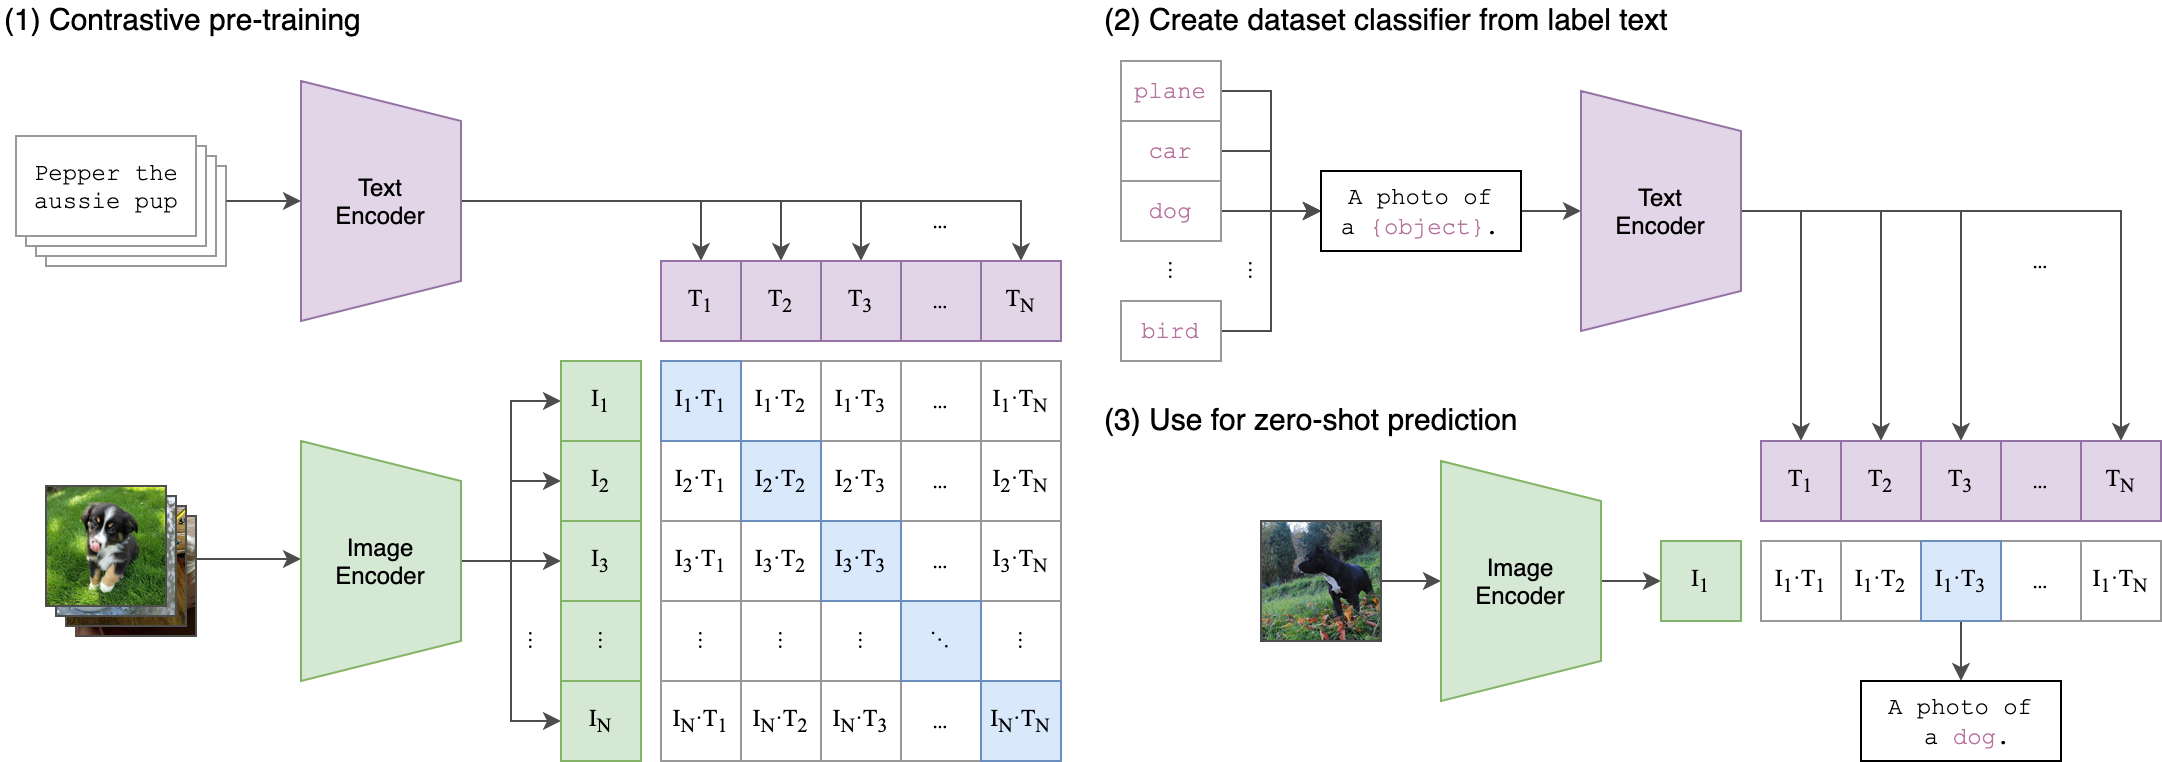
\includegraphics[width=0.82\linewidth]{figures/Contrastive_Language-Image_Pretraining.png}
    \caption{CLIP-style vision-language pretraining aligns image and text representations in a shared embedding space \cite{wikimedia_clip_pretraining_image,radford2021learningtransferablevisualmodels}.}
    \label{fig:intro-vlm-pretraining}
\end{figure}

However, high-performing VLMs are often large and expensive in memory, latency and deployment cost, which limits their use in resource-constrained settings \cite{alayrac2022flamingovisuallanguagemodel,li2023blip2bootstrappinglanguageimagepretraining,chu2023mobilevlm,zhou2024tinyllava}. This issue is especially important for text-centric tasks such as scene-text reading, document understanding and chart reasoning \cite{singh2019vqamodelsread,mathew2021docvqadatasetvqadocument,masry2022chartqabenchmarkquestionanswering}.

\begin{figure}[htbp]
    \centering
    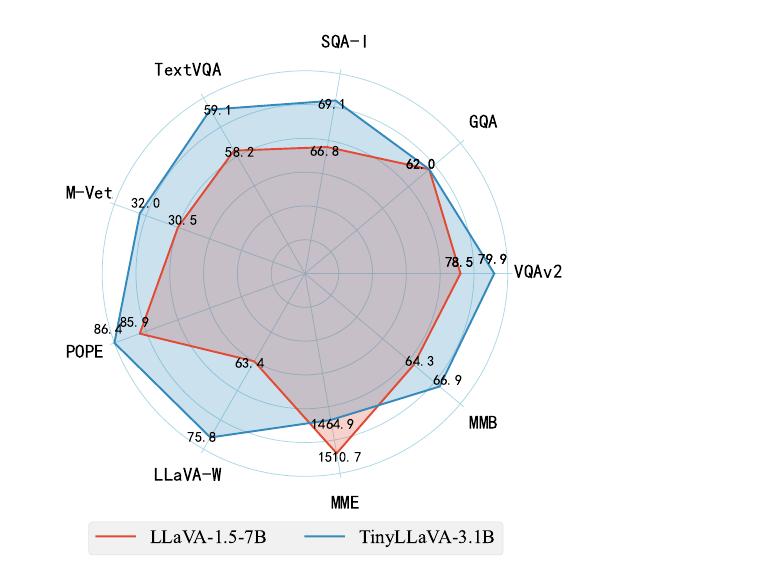
\includegraphics[width=0.66\linewidth]{figures/tinyllava_vs_llava7b_chart.png}
    \caption[TinyLLaVA vs. LLaVA-1.5-7B benchmark comparison.]{Benchmark comparison from TinyLLaVA Figure 1, where a 3.1B small-scale multimodal model remains competitive with the 7B LLaVA-1.5 baseline across several benchmarks \cite{zhou2024tinyllava}.}
    \label{fig:intro-small-vlm-tradeoff}
\end{figure}

Knowledge distillation transfers knowledge from a large teacher to a compact student, achieving competitive performance at lower cost \cite{hinton2015distillingknowledgeneuralnetwork,xu2024surveyknowledgedistillationlarge}. Figure \ref{fig:intro-small-vlm-tradeoff} illustrates why this direction matters: compact multimodal models can remain competitive, but closing the gap to stronger models still requires better transfer of knowledge. In the multimodal setting, recent work has also shown that distillation can be used to transfer reasoning or representation knowledge into more efficient VLMs \cite{hu2024visualprogramdistillation,yang2024clipcid}. For VLMs, this is especially relevant on text-rich benchmarks such as TextVQA, DocVQA and ChartQA \cite{singh2019vqamodelsread,mathew2021docvqadatasetvqadocument,masry2022chartqabenchmarkquestionanswering}.

\begin{figure}[htbp]
    \centering
    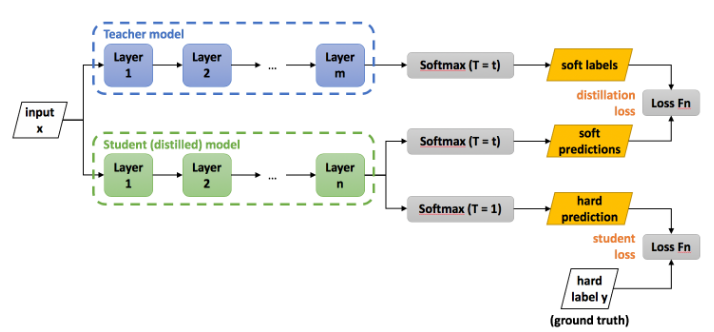
\includegraphics[width=0.70\linewidth]{figures/knowledge_distillation_example.png}
    \caption{Knowledge distillation transfers information from a teacher model to a smaller student model \cite{wikimedia_knowledge_distillation_example,hinton2015distillingknowledgeneuralnetwork}.}
    \label{fig:intro-knowledge-distillation}
\end{figure}

Since no single teacher excels across all multimodal tasks, \textit{multi-teacher distillation} uses multiple complementary teachers with adaptive selection to provide richer, task-relevant supervision \cite{xu2024surveyknowledgedistillationlarge,yuan2020reinforcedmultiteacherselection,zhang2023adaptivemultiteachermetalearning}.

Beyond improving student performance, this thesis also addresses a meta-level problem: \textit{how to choose the right set of teachers for a specific student}. Prior work has shown that fixed or uniform teacher assignment is often suboptimal and recent studies have started to explore adaptive teacher weighting or selective teacher transfer \cite{yuan2020reinforcedmultiteacherselection,zhang2023adaptivemultiteachermetalearning,yu2024selectdistill}. \textbf{To the best of our knowledge, student-specific teacher-set optimization for multimodal VLM distillation remains a completely unexplored problem in the literature.} In this thesis, teacher selection is treated as part of the learning problem itself rather than as a fixed design choice.

This thesis investigates knowledge distillation for VLMs, focusing on how a compact student can learn from multiple teacher VLMs and how teacher-set optimization improves transfer on text-rich multimodal understanding tasks such as reading image text and solving basic reasoning questions in TextVQA, DocVQA and ChartQA \cite{singh2019vqamodelsread,mathew2021docvqadatasetvqadocument,masry2022chartqabenchmarkquestionanswering}.

\section{Problem Statement and Research Objectives}
The central problem addressed in this thesis is how to transfer multimodal understanding ability from large VLMs to compact student models without incurring the full cost of large-scale deployment. In particular, we focus on text-rich multimodal tasks where the student must read image text, understand the question and perform basic reasoning. Existing distillation pipelines usually assume either a single teacher or a fixed set of teachers, which leaves open the harder question of how to select the most useful teachers for a given student model.

Given a pool of \(N\) teacher VLMs and a fixed compact student, the goal is to select \(K\) optimal teachers and train the student to maximize knowledge transfer.

Accordingly, this thesis has three main objectives:
\begin{enumerate}
\item formulate multimodal knowledge distillation for compact VLM students in a text-centric benchmark setting,
\item design an adaptive multi-teacher strategy that treats teacher-set selection as part of the learning problem,
\item evaluate whether teacher-set optimization improves transfer for small VLMs on TextVQA, DocVQA and ChartQA.
\end{enumerate}

\section{Thesis Contributions}
The main contributions of this thesis are summarized as follows:
\begin{enumerate}
\item We formulate student-specific teacher-set optimization for multimodal VLM distillation, focusing on compact students for text-rich multimodal understanding.
\item We propose an adaptive multi-teacher distillation framework in which teacher selection and knowledge transfer are optimized jointly.
\item We study the method on small VLM students and evaluate it on TextVQA, DocVQA and ChartQA using a unified evaluation pipeline.
\end{enumerate}

\section{Thesis Outline}
The remainder of this thesis is organized as follows:
\begin{enumerate}
\item Chapter~\ref{chap:preliminaries} reviews the background on Transformers, VLMs, knowledge distillation and mixture of experts.
\item Chapter~\ref{chap:proposed-method} presents the proposed method, including the problem formulation, teacher selection strategy and training procedure.
\item Chapter~\ref{chap:evaluation-methodology} describes the experimental setup, datasets, evaluation metrics and compared methods.
\item Chapter~\ref{chap:experiment-results} reports the baseline results, comparison results, ablation studies and discussion.
\end{enumerate}
\newpage\cleardoublepage
\chapter{Preliminaries}
\label{chap:preliminaries}

\section{Transformer-Based Vision-Language Models}

\subsection{Transformer Basics}

Modern vision-language models are built on the Transformer architecture
\cite{vaswani2023attentionneed}. For an input sequence, self-attention maps query,
key and value matrices \(\mathbf{Q}\), \(\mathbf{K}\) and \(\mathbf{V}\) to
\begin{equation}
\mathrm{Attention}(\mathbf{Q},\mathbf{K},\mathbf{V})
=
\mathrm{softmax}\!\left(\frac{\mathbf{Q}\mathbf{K}^{\top}}{\sqrt{d_k}}\right)\mathbf{V},
\end{equation}
where \(d_k\) is the key dimension. Multi-head attention runs this operation
in parallel across several learned subspaces, then applies a feed-forward
network and residual normalization.

For language modeling, the Transformer produces a sequence of hidden states and
next-token logits. In this thesis, the student and teacher interact through
their output logits because the distillation method operates at the
token-distribution level \cite{vaswani2023attentionneed,hinton2015distillingknowledgeneuralnetwork}.

\begin{figure}[tp]
    \centering
    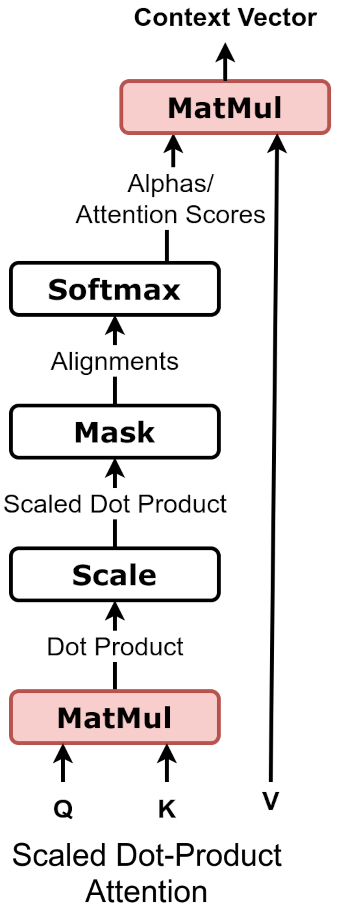
\includegraphics[height=0.20\textheight,keepaspectratio]{figures/transformer_attention_block_wikimedia.png}
    \caption{Transformer attention block structure \cite{wikimedia_transformer_attention_block_image,vaswani2023attentionneed}. The figure isolates the attention and feed-forward block that is later reused in both language and vision stacks.}
    \label{fig:prelim-transformer-attention}
\end{figure}

\subsection{Vision Encoder and Multimodal Fusion}

On the visual side, many multimodal systems use a Vision Transformer (ViT)
\cite{dosovitskiy2021imageworth16x16words}, which converts an image into a sequence
of patch embeddings and processes them with Transformer blocks. A connector
module then fuses these visual tokens with text, using cross-attention, a Q-Former,
or a learned projector
\cite{alayrac2022flamingovisuallanguagemodel,li2023blip2bootstrappinglanguageimagepretraining,liu2023visualinstructiontuning}.

This thesis focuses on compact generative VLMs in the same general family as
SmolVLM and related projector-based models. Conceptually, we can write such a model as
\begin{equation}
\mathbf{z} = f_{\theta}(x),
\end{equation}
where \(x\) is a multimodal input and \(\mathbf{z}\) denotes the output logits
used for autoregressive answer generation.

\begin{figure}[tp]
    \centering
    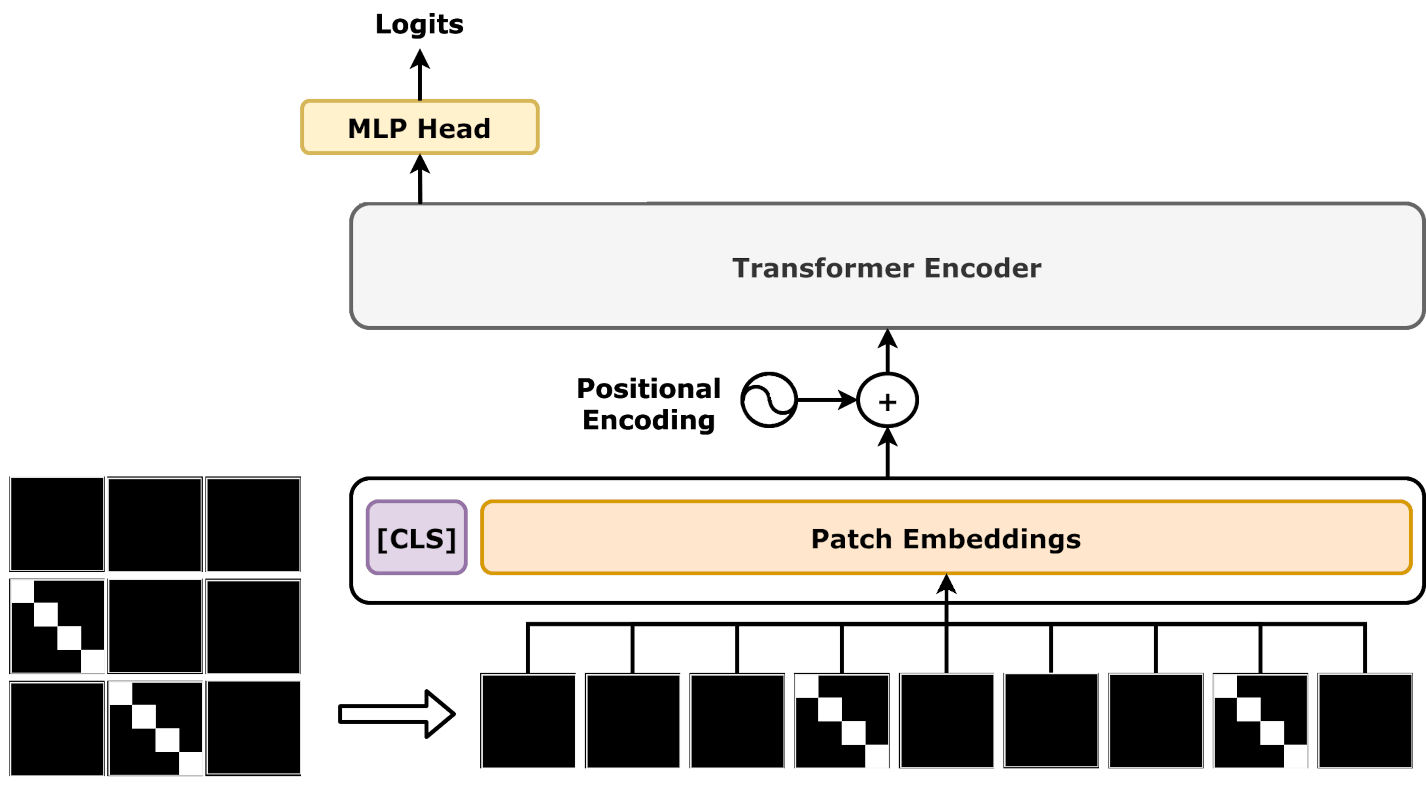
\includegraphics[width=0.68\linewidth]{figures/vit_wikimedia.png}
    \caption{Vision Transformer pipeline with patch embedding and Transformer encoder blocks \cite{wikimedia_vision_transformer_image,dosovitskiy2021imageworth16x16words}. It shows how an image becomes a token sequence before multimodal fusion.}
    \label{fig:prelim-vit}
\end{figure}

Figures~\ref{fig:prelim-transformer-attention} and \ref{fig:prelim-vit} give
the basic Transformer and ViT blocks that later multimodal systems build on.

\begin{figure}[tp]
    \centering
    \begin{subfigure}[t]{0.48\linewidth}
        \centering
        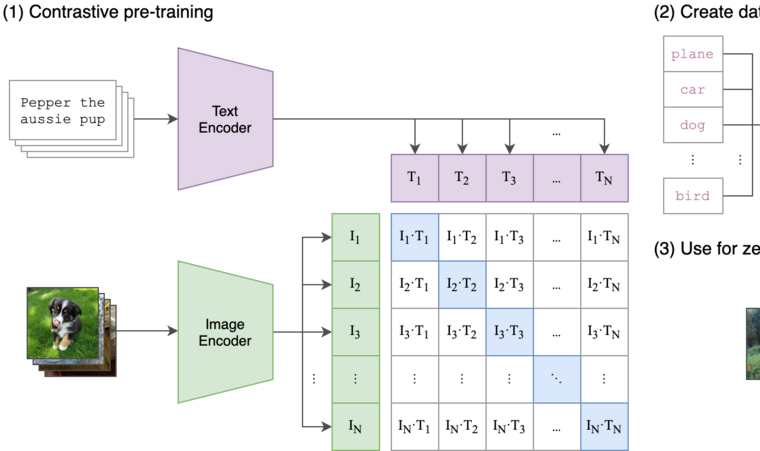
\includegraphics[width=\linewidth]{figures/clip_architecture_family.png}
        \caption{CLIP-style dual encoder \cite{radford2021learningtransferablevisualmodels}.}
    \end{subfigure}
    \hfill
    \begin{subfigure}[t]{0.48\linewidth}
        \centering
        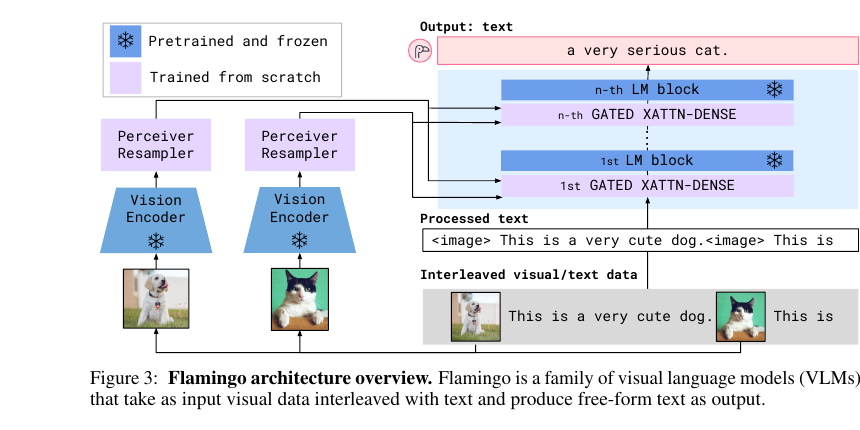
\includegraphics[width=\linewidth]{figures/flamingo_architecture_family.png}
        \caption{Flamingo cross-attention design \cite{alayrac2022flamingovisuallanguagemodel}.}
    \end{subfigure}

    \vspace{0.6em}

    \begin{subfigure}[t]{0.48\linewidth}
        \centering
        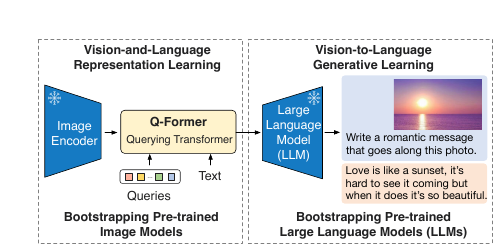
\includegraphics[width=\linewidth]{figures/blip2_architecture_family.png}
        \caption{BLIP-2 with Q-Former \cite{li2023blip2bootstrappinglanguageimagepretraining}.}
    \end{subfigure}
    \hfill
    \begin{subfigure}[t]{0.48\linewidth}
        \centering
        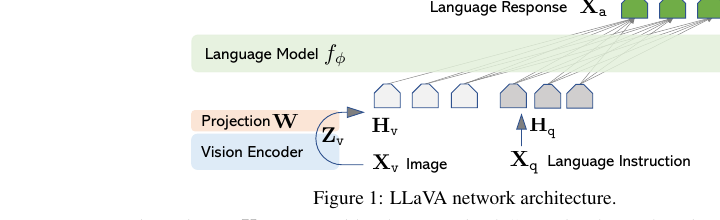
\includegraphics[width=\linewidth]{figures/llava_architecture_family.png}
        \caption{LLaVA projector-based design \cite{liu2023visualinstructiontuning}.}
    \end{subfigure}
    \caption{Representative architecture families of modern vision-language models. Together they show the main fusion choices used in practice: dual encoders, cross-attention, query bottlenecks and projector-based coupling to a language model.}
    \label{fig:prelim-vlm-families}
\end{figure}

\subsection{Text-Rich Multimodal Understanding}

The tasks considered in this thesis, namely TextVQA, DocVQA and ChartQA, require
the model to read text in images, understand the question and perform basic
reasoning over visual and textual evidence
\cite{singh2019vqamodelsread,mathew2021docvqadatasetvqadocument,masry2022chartqabenchmarkquestionanswering}.
This setting differs from generic image captioning because success depends strongly
on optical character recognition (OCR)-sensitive recognition and token-level answer generation.

\begin{figure}[tp]
    \centering
    \begin{subfigure}[t]{0.31\linewidth}
        \centering
        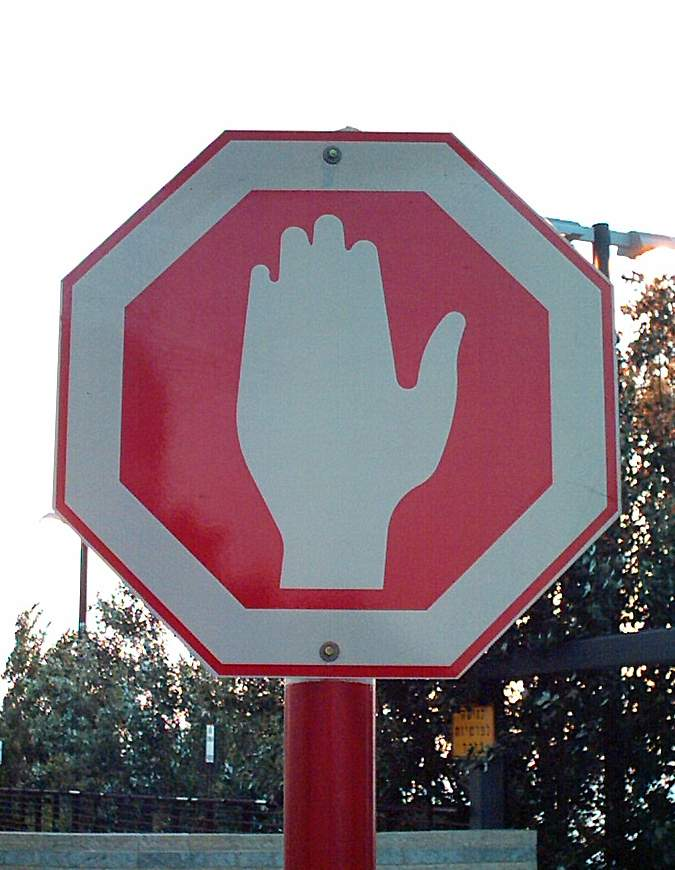
\includegraphics[width=\linewidth,height=0.18\textheight,keepaspectratio]{figures/textvqa_sample_stop_sign.jpg}
        \caption{TextVQA}
    \end{subfigure}
    \hfill
    \begin{subfigure}[t]{0.31\linewidth}
        \centering
        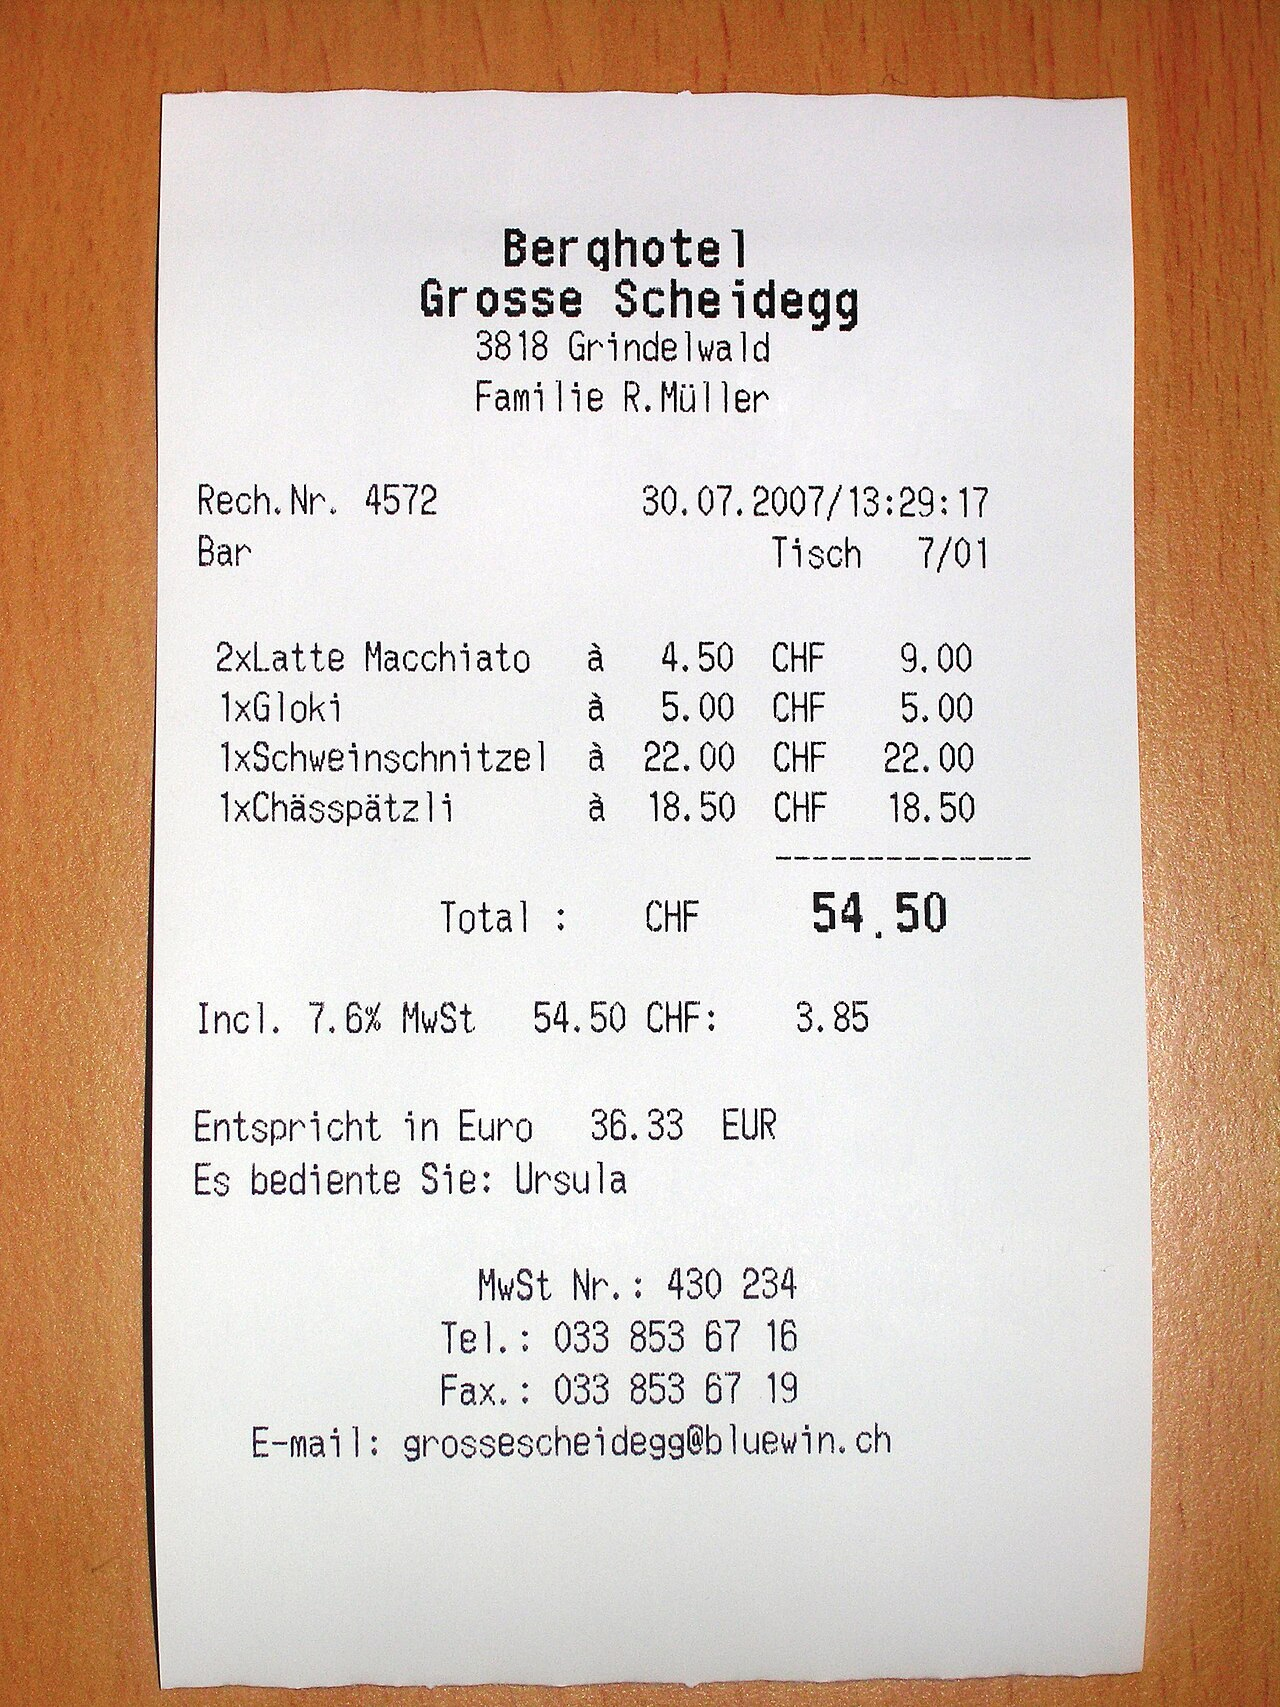
\includegraphics[width=\linewidth,height=0.18\textheight,keepaspectratio]{figures/docvqa_sample_receipt.jpg}
        \caption{DocVQA}
    \end{subfigure}
    \hfill
    \begin{subfigure}[t]{0.31\linewidth}
        \centering
        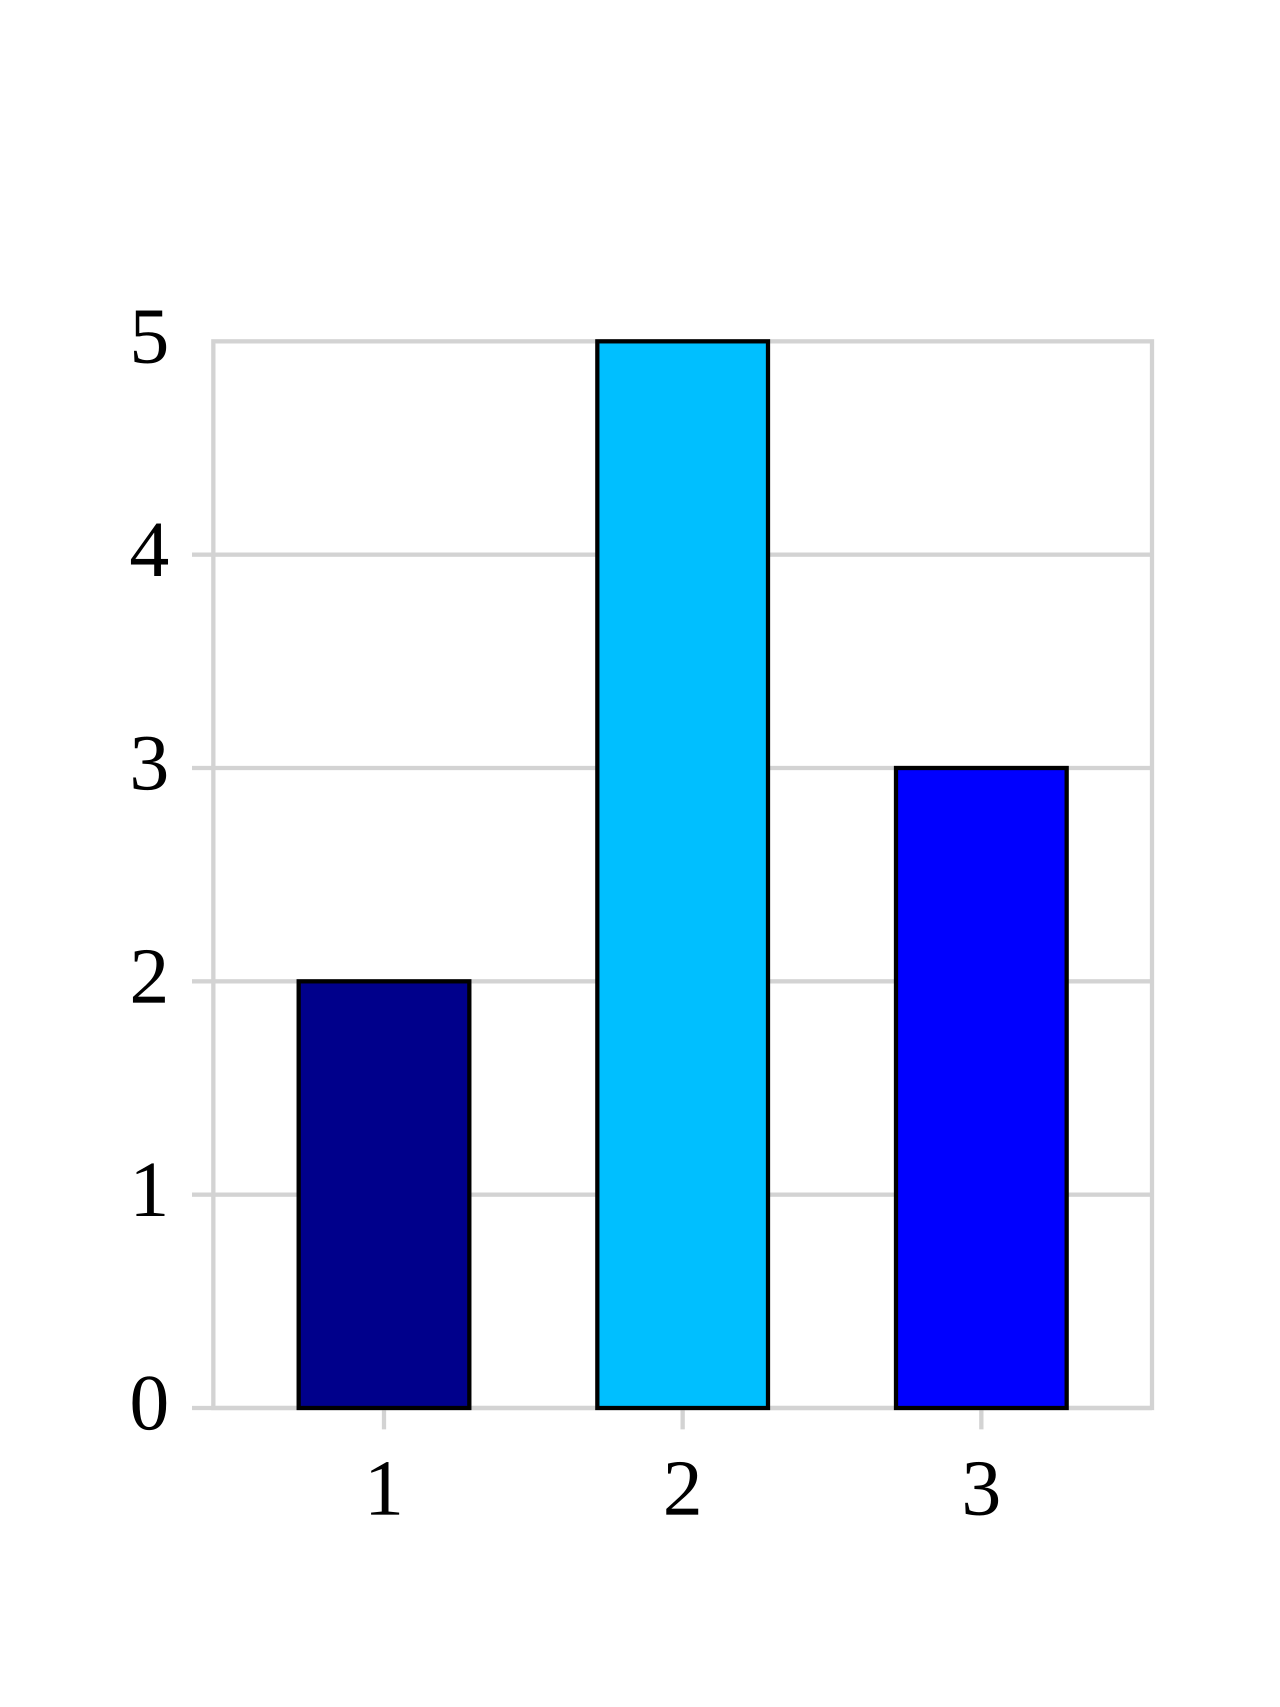
\includegraphics[width=\linewidth,height=0.18\textheight,keepaspectratio]{figures/chartqa_sample_bar_chart.png}
        \caption{ChartQA}
    \end{subfigure}
    \caption{Representative inputs from the text-rich multimodal benchmarks considered in this thesis \cite{singh2019vqamodelsread,mathew2021docvqadatasetvqadocument,masry2022chartqabenchmarkquestionanswering}. The three examples show why text reading, layout parsing and visual reasoning all matter in this benchmark suite.}
    \label{fig:prelim-benchmark-examples}
\end{figure}

Figure~\ref{fig:prelim-vlm-families} summarizes the main architecture families,
while Figure~\ref{fig:prelim-benchmark-examples} shows the text-rich inputs
used in this thesis.

\section{Knowledge Distillation}

\subsection{Teacher-Student Learning}

Knowledge distillation transfers information from a stronger teacher model to a
smaller student model \cite{hinton2015distillingknowledgeneuralnetwork,xu2024surveyknowledgedistillationlarge}.
Let \(\mathcal{L}_{CE}\) denote the supervised cross-entropy loss of the student.
A generic distillation objective takes the form
\begin{equation}
\mathcal{L}
=
\lambda_{CE}\mathcal{L}_{CE}
+
\lambda_{KD}\mathcal{L}_{KD},
\end{equation}
where \(\mathcal{L}_{KD}\) is a teacher-guided loss. In later chapters, GRACE
instantiates this template with a routed trie-Wasserstein term plus small router
regularizers.

In token-level distillation, the teacher and student are compared on their output
logits, not only on hard labels. This allows the student to learn richer
distributional structure, often called \emph{dark knowledge} \cite{hinton2015distillingknowledgeneuralnetwork}.

\begin{figure}[tp]
    \centering
    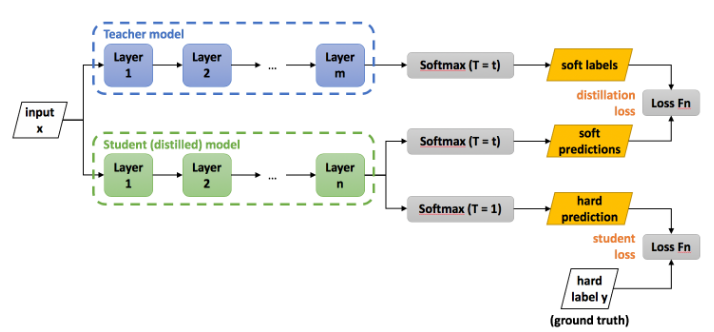
\includegraphics[width=0.78\linewidth]{figures/knowledge_distillation_example.png}
    \caption{Generic teacher-student knowledge distillation setup with hard labels and soft targets \cite{wikimedia_knowledge_distillation_example,hinton2015distillingknowledgeneuralnetwork}. It provides the basic supervision pattern before GRACE adds heterogeneous teachers and routing.}
    \label{fig:prelim-kd-overview}
\end{figure}

Figure~\ref{fig:prelim-kd-overview} provides the generic teacher-student
template before Chapter~\ref{chap:proposed-method} specializes it to GRACE.

\subsection{Temperature-Scaled Output Distributions}

Let \(\mathbf{z}_s\) and \(\mathbf{z}_t\) denote student and teacher logits.
With temperatures \(\tau_s\) and \(\tau_t\), the corresponding distributions are
\begin{equation}
\mathbf{p}_s = \mathrm{softmax}\!\left(\frac{\mathbf{z}_s}{\tau_s}\right),
\qquad
\mathbf{p}_t = \mathrm{softmax}\!\left(\frac{\mathbf{z}_t}{\tau_t}\right).
\end{equation}

Many classical KD methods compare \(\mathbf{p}_s\) and \(\mathbf{p}_t\) using
divergences such as forward KL or Jensen-Shannon divergence. However, such
approaches usually assume that teacher and student share the same vocabulary
\cite{hinton2015distillingknowledgeneuralnetwork,lin1991jensen,boizard2024towardscrosstokenizerdistillation}.

\section{Cross-Tokenizer Distillation Background}

\subsection{Motivation}

In this thesis, the teacher pool may contain different VLM families with
different tokenizers and vocabulary sizes. A KD loss that assumes a shared
output space is therefore too restrictive. Universal Logit Distillation (ULD)
is one important prior remedy because it avoids direct token-ID matching
\cite{boizard2024towardscrosstokenizerdistillation}. Chapter~\ref{chap:proposed-method}
later replaces the ranked-mass surrogate with a trie-Wasserstein variant that
keeps the same cross-tokenizer goal but uses a tree-structured transport view.

\begin{figure}[tp]
    \centering
    \includegraphics[width=0.58\linewidth]{figures/uld_vocab_overlap.png}
    \caption{Vocabulary-overlap ratios between teacher and student tokenizers from the ULD paper \cite{boizard2024towardscrosstokenizerdistillation}. The overlap is far from complete, which makes direct token-ID KD unreliable across model families.}
    \label{fig:prelim-uld-overlap}
\end{figure}

Figure~\ref{fig:prelim-uld-overlap} makes the mismatch explicit: even strong
teacher-student pairs can share only part of their vocabularies.

\subsection{ULD as a Prior Baseline}

Given student logits \(\mathbf{z}_s \in \mathbb{R}^{V_s}\) and teacher logits
\(\mathbf{z}_t \in \mathbb{R}^{V_t}\), we first compute their temperature-scaled
probability distributions \(\mathbf{p}_s\) and \(\mathbf{p}_t\). We then sort both
vectors in descending order, pad the smaller vocabulary with zeros and compare
the sorted masses with an \(L_1\) distance:
\begin{equation}
\mathcal{L}_{ULD}(\mathbf{z}_s,\mathbf{z}_t)
=
\left\|
\pi(\mathbf{p}_s)-\pi(\mathbf{p}_t)
\right\|_1,
\end{equation}
where \(\pi(\cdot)\) denotes sorting in descending order after zero-padding.

The key advantage of ULD is that it compares distributions by ranked
probability mass instead of token identity. This makes it directly
applicable to cross-tokenizer teacher-student distillation
\cite{boizard2024towardscrosstokenizerdistillation}. In the later experiments,
ULD is treated as a cross-tokenizer baseline, not the final method.

\begin{figure}[tp]
    \centering
    \includegraphics[width=0.88\linewidth]{figures/uld_pipeline.png}
    \caption{ULD pipeline from the original paper \cite{boizard2024towardscrosstokenizerdistillation}. Teacher and student probabilities are sorted and zero-padded before the ranked masses are compared, which removes the need for direct vocabulary alignment.}
    \label{fig:prelim-uld-pipeline}
\end{figure}

\subsection{Optimal Transport and Tree-Structured Mass Matching}

Optimal transport compares two probability measures by the minimum cost required
to move mass from one distribution to the other
\cite{peyre2019computationaloptimaltransport}. For discrete source weights
\(\mathbf{a}\), target weights \(\mathbf{b}\) and transport cost matrix
\(\mathbf{C}\), the corresponding optimization problem can be written as
\begin{equation}
W(\mathbf{a},\mathbf{b})
=
\min_{\mathbf{P}\in\mathcal{U}(\mathbf{a},\mathbf{b})}
\langle \mathbf{P}, \mathbf{C} \rangle,
\qquad
\mathcal{U}(\mathbf{a},\mathbf{b})
=
\left\{
\mathbf{P}\ge 0 \mid
\mathbf{P}\mathbf{1}=\mathbf{a},\
\mathbf{P}^{\top}\mathbf{1}=\mathbf{b}
\right\}.
\end{equation}
Here, \(\mathbf{P}\) is a transport plan that specifies how much mass is moved
from each source bin to each target bin.

\begin{figure}[tp]
    \centering
    \includegraphics[width=0.78\linewidth]{figures/continuous_optimal_transport_wikimedia.png}
    \caption{Continuous displacement view of optimal transport \cite{wikimedia_continuous_optimal_transport_image,peyre2019computationaloptimaltransport}. The figure emphasizes the geometric side of OT: mass is moved through space with a transport map, not compared by fixed bin identity alone.}
    \label{fig:prelim-continuous-ot}
\end{figure}

Figure~\ref{fig:prelim-continuous-ot} gives the continuous geometric view of
OT. The same idea appears in the discrete case through a transport plan
\(\mathbf{P}\), and later in the tree case through edgewise subtree mass.

This viewpoint also motivates tree-structured transport. When teacher and
student have different vocabularies, matching probabilities by token index is
not meaningful. What matters instead is how probability mass sits on a
shared structure \cite{boizard2024towardscrosstokenizerdistillation,peyre2019computationaloptimaltransport}.

Tree-Wasserstein distances make that idea explicit by placing probability mass
on a tree metric and summing weighted subtree imbalances
\cite{takezawa2021supervisedtreewasserstein,peyre2019computationaloptimaltransport}.
For a rooted tree \(T=(V,E)\) with edge weights \(w(e)\), one convenient form is
\begin{equation}
W_T(\mu,\nu)
=
\sum_{e\in E}
w(e)\,
\left|
\mu\!\left(\Gamma(e)\right)-\nu\!\left(\Gamma(e)\right)
\right|,
\end{equation}
where \(\Gamma(e)\) denotes the subtree below edge \(e\). The key point is that,
on a tree metric, transport decomposes into edgewise subtree-mass imbalance
instead of a dense source-target coupling
\cite{takezawa2021supervisedtreewasserstein,leyamadafukumizucuturi2019treesliced}.
This is computationally attractive because the comparison follows the tree
structure directly and it is conceptually natural when tokens share prefixes or
other hierarchical relations.

\begin{figure}[tp]
    \centering
    \includegraphics[width=0.78\linewidth]{figures/tree_wasserstein_stw_paper.png}
    \caption{Example tree metrics from Quadtree, tree-sliced Wasserstein (TSW) and supervised tree-Wasserstein (STW) on a synthetic dataset \cite{takezawa2021supervisedtreewasserstein}. The comparison is not a VLM result, but it makes the tree-transport idea explicit: mass is organized along branches of a hierarchy instead of through one dense transport matrix.}
    \label{fig:prelim-tree-ot}
\end{figure}

Tree-sliced OT extends the same idea by averaging Wasserstein distances over
tree metrics and shows that tree metrics preserve the geometric view of OT while
admitting fast closed-form computations
\cite{leyamadafukumizucuturi2019treesliced}. In this thesis, the relevant tree
is not an abstract hierarchy but the shared UTF-8 byte trie induced by teacher
and student decoded single-token strings.

That perspective is closer to the trie-Wasserstein loss used later in
Chapter~\ref{chap:proposed-method}: the method maps tokens to paths on a shared byte
trie and compares mass on edges instead of token index.

\begin{figure}[tp]
    \centering
    \includegraphics[height=0.26\textheight,keepaspectratio]{figures/optimal_transport_matrix_wikimedia.png}
    \caption{Discrete transport plan matrix in optimal transport, showing how source and target marginals are coupled by a transport matrix \cite{wikimedia_optimal_transport_matrix_image,peyre2019computationaloptimaltransport}. The key idea is geometric: mass is compared by how it can be rearranged, not by fixed token identity.}
    \label{fig:prelim-optimal-transport}
\end{figure}

Figures~\ref{fig:prelim-continuous-ot}, \ref{fig:prelim-optimal-transport}
and \ref{fig:prelim-tree-ot} now cover the three views used later in the
thesis: geometric mass movement, discrete transport plans and tree-structured
mass matching. Chapter~\ref{chap:proposed-method} instantiates the third view
with a shared byte trie and a sparse tree-Wasserstein loss.

\subsection{Answer-Token Distillation}

For multimodal question answering, distillation should focus on answer tokens, not prompt tokens \cite{liu2023visualinstructiontuning}.

In our implementation, the code computes KD only on supervised answer positions after masking ignored tokens, optionally removing EOS and truncating student and teacher answer spans to a common length.

In Chapter~\ref{chap:proposed-method}, these sets are denoted by
\(\Omega_b^{CE}\) for CE and \(\Omega_{b,i}^{KD}\) for teacher-specific KD.

This gives a token-aligned distillation signal while remaining compatible with different tokenizers.

\section{Multi-Teacher Distillation}

\subsection{Per-Teacher KD Loss}

Let \(\mathcal{T}=\{T_1,\ldots,T_N\}\) be a pool of frozen teachers. For sample
\(b\), teacher \(T_i\) produces a per-teacher distillation loss
\(\mathcal{L}_{KD}^{(b,i)}\). In principle, one could average these losses uniformly,
\begin{equation}
\mathcal{L}_{KD}^{(b)}
=
\frac{1}{N}\sum_{i=1}^{N}\mathcal{L}_{KD}^{(b,i)},
\end{equation}
but this assumes every teacher is equally useful for every sample.

In practice, different teachers may provide conflicting guidance. Some teachers
may help the supervised objective on a given sample, while others may push the
student in a different direction \cite{zhu2021studentcustomized}. This motivates
a selective routing mechanism that decides, for each sample, which teachers
should be active.

\subsection{Learned Routing and Load Balancing}

Recent sparse expert models route each sample or token through only a subset of available experts. This improves efficiency and allows specialized computation \cite{shazeer2017outrageouslylargeneuralnetworks,fedus2022switchtransformersscalingtrillion,deepseekai2024deepseekv2strongeconomicalefficient}.

The same high-level idea is useful in multi-teacher distillation. Instead of averaging all teachers equally, a learned router can propose teacher weights from student-side features \cite{yuan2020reinforcedmultiteacherselection,zhang2023adaptivemultiteachermetalearning,yu2024selectdistill}.

Let \(\mathbf{h}^{(b)}\) denote a pooled student representation for sample \(b\).
A router network \(G(\cdot)\) produces gate logits
\begin{equation}
\mathbf{r}^{(b)} = G(\mathbf{h}^{(b)}),
\qquad
\tilde{\mathbf{r}}^{(b)} = \text{AdjustedScores}\!\left(\mathbf{r}^{(b)}\right),
\qquad
\mathbf{p}^{(b)} = \mathrm{softmax}\!\left(\tilde{\mathbf{r}}^{(b)}\right),
\end{equation}
where \(p_i^{(b)}\) is the initial routing weight for teacher \(T_i\). In the
current implementation, \(\tilde{\mathbf{r}}^{(b)}\) includes expert bias,
optional training noise and router-temperature scaling before softmax.

In sparse routing, these weights are typically refined by additional constraints:
\begin{enumerate}
\item \textbf{Top-\(k\) routing}, which keeps only the highest-scoring teachers.
\item \textbf{Capacity constraints}, which prevent one teacher from receiving too many assignments.
\item \textbf{Load balancing}, which discourages routing collapse onto a small subset of teachers.
\end{enumerate}

Following the general MoE literature, one can summarize the balancing signal by a
soft load \(\bar{p}_i\) and a hard assignment load \(\bar{q}_i\) after sparse
routing, capacity control and fallback and define an
auxiliary balancing objective of the form
\begin{equation}
\mathcal{L}_{bal}
=
N\sum_{i=1}^{N}\bar{p}_i \bar{q}_i.
\end{equation}
This auxiliary term does not replace the KD objective; instead, it regularizes
the router so that different teachers remain usable during training.

In \methodname, the code implements the router as a small student-conditioned MLP gate on
top of pooled student hidden states. It then applies softmax weights,
top-\(k\) sparsification and capacity filtering, with a short dense warmup
before sparse routing starts. The full framework also supports optional
balancing, entropy regularization and expert-bias updates.

When enabled, the expert bias term nudges the router toward under-used teachers
in subsequent batches.

This makes the routing stage closer to sparse-expert training than to a static teacher average \cite{shazeer2017outrageouslylargeneuralnetworks,fedus2022switchtransformersscalingtrillion,zhou2022mixtureofexpertswithexpertchoice}.

\begin{figure}[tp]
    \centering
    \includegraphics[width=0.80\linewidth]{figures/switch_capacity_routing_jmlr_clean2.png}
    \caption[Sparse routing with expert capacity constraints.]{Illustration of sparse routing with expert capacity constraints, adapted from Switch Transformers \cite{fedus2022switchtransformersscalingtrillion}. Capacity factors control how many routed samples each expert can accept before overflow, which is directly analogous to the capacity-aware teacher routing used in \methodname.}
    \label{fig:prelim-switch-routing}
\end{figure}

The next figure adds the specialization view. Sparse routing does not only save
compute, it also lets different experts focus on different inputs.

\begin{figure}[tp]
    \centering
    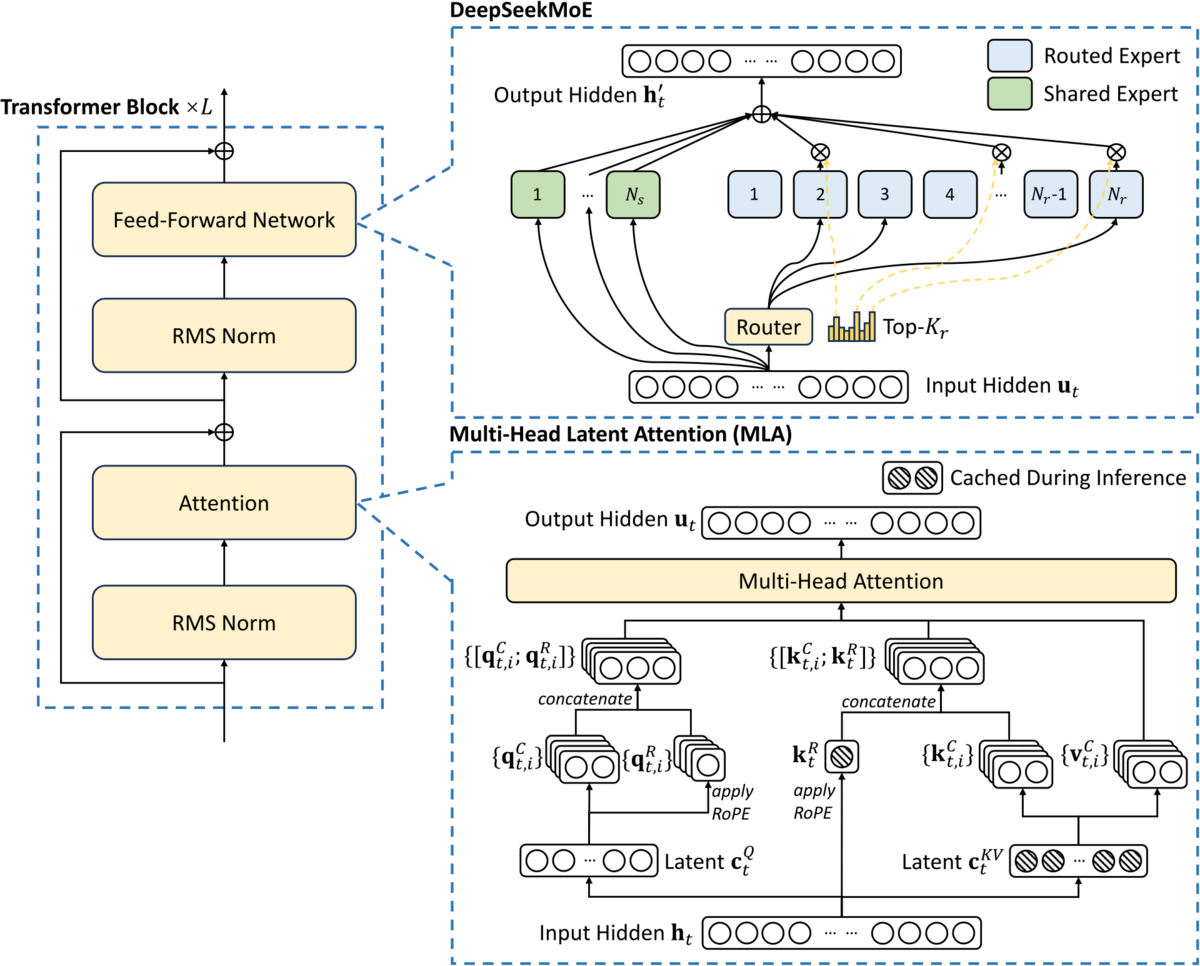
\includegraphics[width=0.78\linewidth]{figures/deepseek_moe_wikimedia.png}
    \caption[Sparse routing and expert specialization in MoE.]{Example of sparse routing and expert specialization in a mixture-of-experts architecture \cite{wikimedia_deepseek_moe_mla_image,deepseekai2024deepseekv2strongeconomicalefficient}. Although our setting is multi-teacher distillation, not token-level MoE language modeling, the same principles of learned routing, sparse activation and load balancing are directly relevant.}
    \label{fig:prelim-sparse-routing}
\end{figure}

Figures~\ref{fig:prelim-switch-routing} and \ref{fig:prelim-sparse-routing}
summarize the sparse-routing ideas that motivate the teacher gate in GRACE.

\subsection{Gradient Alignment as a Routing Signal}

Prior work uses gradient similarity in distillation as a signal for deciding
whether teacher supervision helps or conflicts with the student objective
\cite{zhu2021studentcustomized}. If the teacher-induced update points in a
similar direction to the supervised update, the teacher is more likely to be
helpful. If the two directions conflict, teacher supervision may hurt learning
on that sample \cite{zhu2021studentcustomized}.

In \methodname{}, this idea is applied only after routing. The router first
decides which teachers remain available and Chapter~\ref{chap:proposed-method}
then refines those routed teachers with continuous gradient-based scores. The
GRACE-specific details, including score smoothing, score softmax, router-score
blending and uniform fallback, are therefore deferred to Chapter~\ref{chap:proposed-method}.

\section{Related Work}

\subsection{Compact VLM Distillation and Compression}

Knowledge distillation is a standard way to compress large models into smaller
students while retaining part of the teacher's predictive structure
\cite{hinton2015distillingknowledgeneuralnetwork,xu2024surveyknowledgedistillationlarge}.
In multimodal systems, prior work has used distillation to compress
visual-linguistic models, transfer reasoning behavior, or improve compact
vision-language students
\cite{fang2021compressingvlm,hu2024visualprogramdistillation,yang2024clipcid}.
These studies show that small VLMs can benefit from teacher supervision, but
most of them do not focus on heterogeneous teacher pools with mismatched
tokenizers.

Compression by quantization is also important in practice, but it is a
different intervention point: quantization changes the numerical precision of a
trained model, while distillation changes how the student is trained
\cite{frantar2022gptq,xiao2023smoothquant,lin2024awq,li2025mbq}. This thesis
therefore treats quantization as complementary deployment work and focuses the
method contribution on distillation.

\subsection{Cross-Tokenizer Distillation}

Cross-tokenizer KD becomes necessary when teacher and student vocabularies do
not match. ULD is a direct baseline in this setting because it compares sorted
probability mass instead of token IDs
\cite{boizard2024towardscrosstokenizerdistillation}. More recent work also
studies tokenizer-agnostic distillation through transport-based or alignment
based formulations
\cite{takezawa2021supervisedtreewasserstein,leyamadafukumizucuturi2019treesliced,dasgupta2025improving}.

The main limitation of ranked-mass matching is that it discards structural
relations between decoded token strings. Tree-structured transport retains that
structure by comparing mass on shared branches of a hierarchy
\cite{takezawa2021supervisedtreewasserstein,peyre2019computationaloptimaltransport}.
This is the line of work most relevant to our trie-Wasserstein loss: the
student and teacher are not matched by token ID, but by mass placed on a shared
UTF-8 byte trie.

\subsection{Multi-Teacher Distillation and Adaptive Routing}

Multi-teacher KD has been studied with fixed teacher averages, stochastic
selection and meta-learned weighting rules
\cite{yuan2020reinforcedmultiteacherselection,zhang2023adaptivemultiteachermetalearning,yu2024selectdistill}.
These methods motivate the use of more than one teacher, but they do not solve
the full combination of heterogeneous VLM teachers, tokenizer mismatch, and
sparse routed weighting in one compact-VLM setting.

Sparse routing and load balancing are well established in mixture-of-experts
models
\cite{shazeer2017outrageouslylargeneuralnetworks,fedus2022switchtransformersscalingtrillion,zhou2022mixtureofexpertswithexpertchoice}.
Our teacher gate borrows that routing view, but applies it to teacher
selection, not to internal expert blocks. Gradient-based teacher filtering has
also appeared in distillation through alignment-style objectives
\cite{zhu2021studentcustomized}. \methodname{} combines these ideas in a
two-stage procedure: sparse student-conditioned routing first, then
post-routing GRACE score refinement.

\subsection{Relation to This Thesis}

This thesis sits at the intersection of the three lines above. It studies
compact generative VLM distillation, replaces ranked-mass ULD with a
cross-tokenizer trie-Wasserstein loss in the main method and combines that
loss with sparse multi-teacher routing plus gradient-based score refinement.
Later chapters keep ULD, SHM-CKA and reinforced teacher selection as
baselines, but the final method integrates the transport, routing, and
alignment ideas into one framework.
\newpage\cleardoublepage
\chapter{Proposed Method}
\label{chap:proposed-method}

This chapter presents \textbf{\gracefull{} (\gracename{})} by first defining
the heterogeneous multi-teacher distillation setting, then introducing the
\textbf{trie-Wasserstein KD loss}, \textbf{teacher routing network},
\textbf{gradient-agreement refinement mechanism} and \textbf{final training
objective}.

This chapter is organized as follows.
Section~\ref{sec:method-overview-formulation} introduces the problem
formulation and the overall \methodname{} training flow.
Section~\ref{sec:trie-wasserstein-distillation} presents trie-Wasserstein
distillation for mismatched tokenizers.
Section~\ref{sec:teacher-routing-network} defines the teacher routing network
and sparse top-\(k\) selection.
Section~\ref{sec:gradient-agreement-refinement} introduces gradient-agreement
refinement and the final teacher weighting mechanism.
Section~\ref{sec:final-objective} combines these components into the final
optimization objective.

\methodname{} addresses three core difficulties in heterogeneous
teacher-to-student VLM distillation. \textbf{First}, teacher and student models may use
different tokenizers and output vocabularies, so standard token-index KD is
not directly applicable. \textbf{Second}, teacher usefulness varies across
image-question pairs, making fixed teacher averaging inefficient. \textbf{Third}, even
routed teachers may still produce KD gradients that conflict with the
supervised task objective. \textbf{Finally}, the method developed in this chapter addresses
these issues through trie-Wasserstein KD, sparse teacher routing and
gradient-agreement refinement.

\section{Method Overview and Problem Formulation}
\label{sec:method-overview-formulation}

We consider multimodal understanding tasks that require reading image
text, understanding the question and generating an answer sequence
\cite{singh2019vqamodelsread,mathew2021docvqadatasetvqadocument,masry2022chartqabenchmarkquestionanswering}.
The training set is
\begin{equation}
\mathcal{D}=\{(x_n,y_n)\}_{n=1}^{N_{\mathrm{data}}},
\end{equation}
where \(x_n\) is a multimodal input and \(y_n\) is the target answer sequence.

Let \(S_{\theta}\) denote the student VLM with trainable parameters
\(\theta\), let \(G_{\phi}\) denote the trainable teacher router with
parameters \(\phi\) and let \(\mathcal{T}=\{T_i\}_{i=1}^{N}\) be the frozen
teacher pool. For each sample \(b\), the student produces logits
\(\mathbf{z}_s^{(b)}\) and teacher \(T_i\) provides teacher logits
\(\mathbf{z}_t^{(b,i)}\).
Throughout this chapter, the frozen teachers are treated as tokenizer-specific
experts: each teacher may use a different tokenizer, vocabulary and model
family and the router selects which experts contribute to each training
sample.

\methodname{} avoids a fixed teacher subset by learning
\textbf{sample-dependent sparse assignments} and refining the routed weights
with \textbf{parameter-gradient agreement}.

\begin{figure}[H]
\centering
\includegraphics[width=\linewidth]{figures/GRACE-Architecture.pdf}
\caption[GRACE architecture.]{GRACE architecture. The student produces logits and hidden states, the teacher routing network selects candidate teachers, trie-Wasserstein KD computes per-teacher losses and gradient-agreement refinement produces final KD weights.}
\label{fig:grace-architecture}
\end{figure}

Figure~\ref{fig:grace-architecture} summarizes the full training path. The
method is defined through four operators. \textbf{Trie-Wasserstein KD} computes
per-teacher distillation losses on a shared byte trie. The
\textbf{teacher routing network} selects candidate teachers from student-side
hidden states. \textbf{Gradient-agreement refinement} adjusts routed teacher
weights using parameter-gradient agreement. The \textbf{final objective}
combines supervised CE, routed KD and router auxiliary terms.

GRACE adapts sparse expert routing
\cite{shazeer2017outrageouslylargeneuralnetworks,fedus2022switchtransformersscalingtrillion}
to heterogeneous multi-teacher VLM distillation with token-level logit
supervision \cite{zhu2021studentcustomized}.

Table~\ref{tab:notation} summarizes the main notation used in the method.
Section~\ref{subsec:training-flow} gives a concise overview of one GRACE training update and the
following sections define these operators in detail, moving from
tokenizer-agnostic distribution matching to teacher routing,
gradient-agreement refinement and final loss aggregation.

\subsection{Notation}

\begin{table}[H]
\centering
\caption{Main symbols used in Chapter~\ref{chap:proposed-method}.}
\label{tab:notation}
\small
\begin{tabular}{@{}p{0.26\textwidth}p{0.66\textwidth}@{}}
\toprule
Symbol & Meaning \\
\midrule
\(\mathcal{D}=\{(x_n,y_n)\}_{n=1}^{N_{\mathrm{data}}}\) & Multimodal samples and target answer sequences. \\
\(S_{\theta}\), \(\mathcal{T}=\{T_i\}_{i=1}^{N}\) & Trainable student VLM and frozen teacher pool. \\
\(G_{\phi}\) & Trainable teacher routing network with parameters \(\phi\). \\
\(\mathbf{z}_s^{(b)}\), \(\mathbf{z}_t^{(b,i)}\) & Student and teacher logits for sample \(b\). \\
\(\mathbf{H}_s\), \(\mathbf{h}\) & Student hidden states and pooled routing feature. \\
\(T_{\mathrm{train}}\) & Total number of training steps. \\
\(\rho_{\mathrm{trie}}\), \(K_{\mathrm{TW}}\), \(e_{\mathrm{tail}}\) & Trie edge decay, sparse support size and residual tail edge. \\
\(k_{\mathrm{route}}\) & Configured router top-\(k\). \\
\(\mathbf{r}\), \(\mathbf{p}\) & Router logits and soft router weights. \\
\(\mathcal{C}_b\), \(\mathcal{R}_b\), \(\hat{\mathbf{p}}^{(b)}\) & Top-\(k\) candidate teacher set, routed teacher set and renormalized routed weights. \\
\(s_i\), \(\hat{s}_i\), \(\tilde{a}_i\), \(a_i^{(b)}\), \(\mathcal{A}_b\) & Raw agreement score, EMA-smoothed agreement score, teacher active flag, sample active flag and active routed set. \\
\(\boldsymbol{\omega}^{(b)}\), \(\mathbf{w}^{(b)}\) & Score-softmax weights and final KD weights. \\
\(\Omega_b^{CE}\), \(\Omega_{b,i}^{KD}\) & Supervised CE positions and matched KD positions. \\
\(\mathbf{g}_{CE}\), \(\mathbf{g}_i\) & CE and teacher-KD parameter gradients used by GRACE. \\
\(\beta_{\mathrm{EMA}}\), \(\beta_{\mathrm{score}}\), \(\epsilon_{\mathrm{num}}\), \(\epsilon_{\mathrm{fb}}\), \(\lambda_{\mathrm{blend}}\) & EMA decay, score-softmax sharpness, cosine stabilizer, fallback threshold and router-score blend exponent. \\
\(\mathrm{TopKRoute}\) & Sparse top-\(k\) teacher routing with routed-weight renormalization. \\
\(U\) & Uniform fallback weights over the active routed set. \\
\(\mathrm{Blend}\) & Mixing routed weights with GRACE score weights. \\
\(\mathrm{EMA}\) & Exponential moving average for GRACE scores. \\
\bottomrule
\end{tabular}
\end{table}

Each GRACE update can be viewed as a four-stage training flow:
\textbf{student forward pass}, \textbf{teacher routing},
\textbf{trie-Wasserstein KD computation} and
\textbf{gradient-agreement refinement}. In the first stage, the student
processes the mini-batch to produce answer-token logits \(\mathbf{z}_s\),
hidden states \(\mathbf{H}_s\) and the supervised loss
\(\mathcal{L}_{CE}\). The router then computes gate logits~\(\mathbf r\),
soft routing weights~\(\mathbf p\) and selects teachers with top-\(k\)
masking. The third stage computes per-sample, per-teacher trie-Wasserstein
losses \(\mathcal{L}_{KD}^{(b,i)}\), which provide tokenizer-agnostic KD
signals for the selected teachers. The final stage computes
parameter-gradient agreement scores, smooths them over time, blends them with
the routed weights and applies fallback when needed.

\subsection{Training Flow}
\label{subsec:training-flow}

A GRACE update starts from a mini-batch
\(\mathcal{B}=\{(x_b,y_b)\}_{b=1}^{B}\) and a frozen teacher pool
\(\mathcal{T}=\{T_i\}_{i=1}^{N}\). The student \(S_\theta\) first processes the
multimodal inputs and returns answer-token logits \(\mathbf{z}_s\), hidden
states \(\mathbf{H}_s\) and the supervised loss \(\mathcal{L}_{CE}\). The
supervised answer positions \(\Omega_b^{CE}\) define both the cross-entropy
loss and the pooling region used by the teacher router.

The router pools the student hidden states over supervised answer positions and
maps the resulting feature \(\mathbf{h}^{(b)}\) to teacher scores. After softmax
normalization, top-\(k_{\mathrm{route}}\) masking keeps a small routed teacher
set \(\mathcal{R}_b\) for each sample. The selected teacher weights are
renormalized to obtain \(\hat{\mathbf{p}}^{(b)}\). This stage replaces fixed
teacher averaging with sample-dependent teacher selection.

For each routed teacher, GRACE compares the student answer-token distribution
with the corresponding teacher distribution using trie-Wasserstein KD. In the
implementation used for the experiments, teacher logits are generated offline
and streamed during training, so the online update trains only the student and
router while the teachers remain frozen. This produces a per-sample,
per-teacher KD loss \(\mathcal{L}_{KD}^{(b,i)}\).

During warmup, the final KD weights are the renormalized router weights. After
warmup, GRACE computes a teacher-level agreement score by comparing the
supervised CE gradient with each teacher's batch-level KD gradient. The
agreement scores are smoothed with EMA, intersected with the routed teacher set
and converted into final sample-level KD weights. If no routed teacher passes
the agreement threshold, GRACE falls back to the router weights. If active
scores are nearly tied, it uses uniform active weights. Otherwise, it blends
router weights with gradient-agreement weights.

The mini-batch KD loss is the weighted average of the routed per-teacher losses.
The final objective combines supervised CE, routed trie-Wasserstein KD, router
entropy regularization and router z-loss. The next sections define these
components formally.

\section{Trie-Wasserstein Cross-Tokenizer Distillation}
\label{sec:trie-wasserstein-distillation}

\subsection{Supervised Answer Tokens}

We apply distillation only on \textbf{supervised answer tokens}, not on prompt
tokens.
For sample \(b\), let \(\Omega_b^{CE}\) denote the student positions whose labels
are not ignored. For each teacher \(T_i\), let \(\Omega_{b,i}^{KD}\) denote the
matched answer positions after masking ignored labels on both student and
teacher sides, removing EOS from the student or teacher answer span when configured
and truncating both spans to a common length.


This is a position-wise alignment approximation across tokenizers: after
answer-span preprocessing, the \(j\)-th student and teacher answer positions are
treated as corresponding positions. The trie-Wasserstein term handles
token-distribution mismatch at each matched position, but it does not perform a
separate byte-level sequence alignment.

\subsection{Shared Byte Trie}

For each sample \(b\), token position \(j \in \Omega_{b,i}^{KD}\) and teacher \(T_i\), let
\(\mathbf{z}_{s,j}^{(b)} \in \mathbb{R}^{V_s}\) be the student logits and
\(\mathbf{z}_{t,j}^{(b,i)} \in \mathbb{R}^{V_i}\) be the teacher logits.
The student and teacher probability distributions are
\begin{equation}
\mathbf{p}_{s,j}^{(b)}
=
\mathrm{softmax}\!\left(\frac{\mathbf{z}_{s,j}^{(b)}}{\tau_s}\right),
\qquad
\mathbf{p}_{t,j}^{(b,i)}
=
\mathrm{softmax}\!\left(\frac{\mathbf{z}_{t,j}^{(b,i)}}{\tau_t}\right),
\end{equation}
where \(\tau_s\) and \(\tau_t\) are the student and teacher temperatures.

Teacher and student vocabularies may differ, so direct token-index matching is
not feasible. GRACE instead maps decoded teacher and student token strings
into a \textbf{shared UTF-8 byte trie}. Tokens with common byte prefixes share
the same initial trie path, even when their tokenizer IDs differ.

Using UTF-8 bytes is a necessary design choice because it provides a fixed alphabet and exposes
tokenizer artifacts such as leading spaces, wordpiece prefixes and multimodal
special tokens. Character-level matching is less stable because the same
visible text can be stored with different Unicode code-point sequences.

For example, a string with a \textbf{leading space maps} to byte sequence
\([32,99,97,116]\), while \texttt{cat} maps to \([99,97,116]\). The trie
therefore treats the leading-space byte as an \textbf{explicit edge}, while
\textbf{preserving the subsequent byte sequence} for the underlying word.

Each token string is converted to a byte sequence and terminated with an EOS
sentinel. The EOS marker separates complete tokens from strict prefixes, so
tokens such as \texttt{doc} and \texttt{document} remain distinct leaves even
though they share an initial path.

Let \(e\) denote a normal byte-trie or EOS edge and let \(d(e)\) be its depth.
GRACE assigns edge weights
\begin{equation}
w(e)=\rho_{\mathrm{trie}}^{d(e)-1},
\label{eq:tw_edge_weight}
\end{equation}
where \(0<\rho_{\mathrm{trie}}<1\). The first edge from the root has weight
\(1\) and deeper edges decay geometrically. This makes shared prefixes cheaper
than unrelated byte paths while preserving a valid tree metric
\cite{takezawa2021supervisedtreewasserstein,peyre2019computationaloptimaltransport}.

Different tokenizers may stop at different depths, but they still share the
same byte-prefix edges when their decoded token strings overlap in byte-prefix
structure. The example in Figure~\ref{fig:grace-trie-shared} uses the pair
\texttt{document}/\texttt{receipt} and \texttt{doc}/\texttt{rece}.

\begin{figure}[H]
\centering
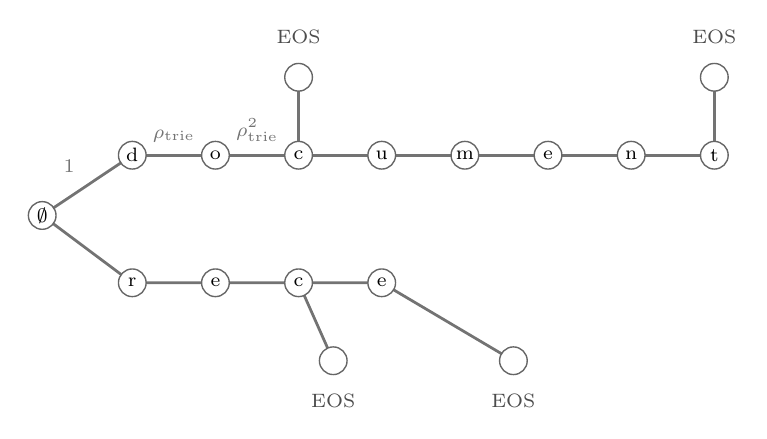
\begin{tikzpicture}[
    x=0.88cm,
    y=0.9cm,
    every node/.style={font=\small},
    every label/.style={fill=white, inner sep=1pt},
    triemark/.style={circle, draw=black!60, fill=white, line width=0.5pt, inner sep=0pt, minimum size=10pt},
    edge/.style={draw=black!55, line width=1.0pt}
]
    \coordinate (root) at (1.8, 2.4);
    \coordinate (d) at (3.1, 3.25);
    \coordinate (o) at (4.3, 3.25);
    \coordinate (c) at (5.5, 3.25);
    \coordinate (u) at (6.7, 3.25);
    \coordinate (m) at (7.9, 3.25);
    \coordinate (e) at (9.1, 3.25);
    \coordinate (n) at (10.3, 3.25);
    \coordinate (t) at (11.5, 3.25);

    \coordinate (r) at (3.1, 1.45);
    \coordinate (e2) at (4.3, 1.45);
    \coordinate (c2) at (5.5, 1.45);
    \coordinate (e3) at (6.7, 1.45);

    \coordinate (eosdoc) at (5.5, 4.35);
    \coordinate (eosdocument) at (11.5, 4.35);
    \coordinate (eosrece) at (6.0, 0.35);
    \coordinate (eosreceipt) at (8.6, 0.35);

    \draw[edge] (root) to node[midway, above left=1pt, font=\scriptsize, text=black!55] {1} (d);
    \draw[edge] (d) to node[midway, above=1pt, font=\scriptsize, text=black!55] {\(\rho_{\mathrm{trie}}\)} (o);
    \draw[edge] (o) to node[midway, above=1pt, font=\scriptsize, text=black!55] {\(\rho_{\mathrm{trie}}^2\)} (c);
    \draw[edge] (c) to (u) to (m) to (e) to (n) to (t);
    \draw[edge] (c) to (eosdoc);
    \draw[edge] (t) to (eosdocument);

    \draw[edge] (root) to (r) to (e2) to (c2) to (e3);
    \draw[edge] (c2) to (eosrece);
    \draw[edge] (e3) to (eosreceipt);

    \foreach \p/\lbl in {
        root/$\emptyset$, d/d, o/o, c/c, u/u, m/m, e/e, n/n, t/t,
        r/r, e2/e, c2/c, e3/e
    }{
        \node[triemark] at (\p) {\scriptsize \lbl};
    }

    \node[triemark, label={[font=\scriptsize, text=black!70, label distance=2mm]above:EOS}] at (eosdoc) {};
    \node[triemark, label={[font=\scriptsize, text=black!70, label distance=2mm]above:EOS}] at (eosdocument) {};
    \node[triemark, label={[font=\scriptsize, text=black!70, label distance=2mm]below:EOS}] at (eosrece) {};
    \node[triemark, label={[font=\scriptsize, text=black!70, label distance=2mm]below:EOS}] at (eosreceipt) {};

\end{tikzpicture}
\caption{Shared-trie view of tokenizer-mismatched matching for \texttt{document}/\texttt{receipt} and \texttt{doc}/\texttt{rece}.}
\label{fig:grace-trie-shared}
\end{figure}

Figure~\ref{fig:grace-trie-shared} illustrates this effect: shorter teacher
token sequences terminate earlier at EOS, whereas longer student token
sequences extend farther down the trie. As a result, the mismatch is
represented through the trie hierarchy instead of direct token-ID comparison.

\subsection{Trie-Wasserstein Objective}

The shared byte trie induces a tree metric over decoded token strings. Let
\(\mathcal{V}_s\) and \(\mathcal{V}_t\) denote the student and teacher token
vocabularies being compared at a given answer position and let \(\pi(v)\)
denote the trie path of decoded token \(v\). For an edge \(e\), the student
and teacher subtree masses are
\[
m_s(e)
=
\sum_{\substack{v\in\mathcal{V}_s\\ e\in\pi(v)}} p_s(v),
\qquad
m_t(e)
=
\sum_{\substack{u\in\mathcal{V}_t\\ e\in\pi(u)}} p_t(u).
\]
Thus, \(m_s(e)\) and \(m_t(e)\) measure how much probability mass each
distribution assigns to token paths passing through edge \(e\). The \(W_1\)
optimal transport distance between teacher and student token distributions on
the trie can then be written as a weighted sum of subtree-mass imbalances:
\begin{equation}
W_T(p_s,p_t)
=
\sum_{e\in E}
w(e)\left|m_s(e)-m_t(e)\right|.
\label{eq:trie-wasserstein-objective}
\end{equation}
This result follows from the standard \(W_1\) Kantorovich optimal transport
formulation under the trie-induced tree metric
\cite{peyre2019computationaloptimaltransport,takezawa2021supervisedtreewasserstein}.
The sparse construction below
applies the same formula to a bounded top-\(K_{\mathrm{TW}}\) support with a
residual tail edge.

\subsection{Sparse Support and Residual Tail Edge}

Equation~\eqref{eq:trie-wasserstein-objective} is exact on the complete shared trie, but
evaluating all vocabulary tokens at every answer position is expensive. GRACE
therefore applies the same subtree-mass formula on a \textbf{sparse augmented trie}.
For each aligned answer position, the method first masks ignored vocabulary
entries and retains the \textbf{top-\(K_{\mathrm{TW}}\) student and teacher tokens}.
These retained tokens are inserted into the shared UTF-8 byte trie while
preserving their exact trie paths and shared prefix structure. The probability
mass assigned to all remaining non-top-\(K_{\mathrm{TW}}\) tokens is not
discarded. Instead, it is collapsed into a single \textbf{residual tail edge}. The
trie-Wasserstein loss is then computed on the augmented structure containing
the retained token paths and the residual tail edge. This construction is
exact for the collapsed sparse trie, but it approximates the complete trie
distance because all omitted vocabulary mass is represented by one tail atom.

Let \(K_{\mathrm{TW}}\) denote the sparse trie support size. Let
\(\mathcal{V}_s^\star\) and \(\mathcal{V}_t^\star\) denote the non-ignored
student and teacher vocabularies. Before constructing the sparse trie, the
student and teacher probabilities are renormalized over the non-ignored
vocabularies so that the retained and residual masses form valid
distributions. Let
\(\mathcal{K}_{s,j}^{(b)}\subset\mathcal{V}_s^\star\) and
\(\mathcal{K}_{t,j}^{(b,i)}\subset\mathcal{V}_t^\star\) be the retained token
sets. The residual mass assigned to the tail edge is
\begin{equation}
r_{s,j}^{(b)}
=
1-\sum_{v\in\mathcal{K}_{s,j}^{(b)}}p_{s,j}^{(b)}(v),
\qquad
r_{t,j}^{(b,i)}
=
1-\sum_{v\in\mathcal{K}_{t,j}^{(b,i)}}p_{t,j}^{(b,i)}(v).
\end{equation}

Let \(\pi(v)\) be the trie path for token \(v\) and let
\(e_{\mathrm{tail}}\) be the global residual tail edge with
\(w(e_{\mathrm{tail}})=1\). For any active trie edge \(e\), the sparse subtree
masses are
\begin{equation}
m_{s,j}^{(b)}(e)
=
\sum_{\substack{v\in\mathcal{K}_{s,j}^{(b)}\\e\in\pi(v)}}
p_{s,j}^{(b)}(v)
\;+\;
\mathbf{1}[e=e_{\mathrm{tail}}]\,r_{s,j}^{(b)},
\end{equation}
\begin{equation}
m_{t,j}^{(b,i)}(e)
=
\sum_{\substack{v\in\mathcal{K}_{t,j}^{(b,i)}\\e\in\pi(v)}}
p_{t,j}^{(b,i)}(v)
\;+\;
\mathbf{1}[e=e_{\mathrm{tail}}]\,r_{t,j}^{(b,i)}.
\end{equation}
The token-level trie-Wasserstein loss is then
\begin{equation}
\ell_{TW}\!\left(\mathbf{z}_{s,j}^{(b)},\mathbf{z}_{t,j}^{(b,i)}\right)
=
\sum_{e\in\mathcal{E}_{act,j}^{(b,i)}}
w(e)\,
\left|
m_{s,j}^{(b)}(e)-m_{t,j}^{(b,i)}(e)
\right|,
\label{eq:token_tw}
\end{equation}
where \(\mathcal{E}_{act,j}^{(b,i)}\) contains the active student edges, active
teacher edges and the residual tail edge. Before the absolute value is applied,
\(m_{s,j}^{(b)}(e)-m_{t,j}^{(b,i)}(e)\) is positive when edge \(e\) carries more
student mass and negative when it carries more teacher mass.

The per-sample, per-teacher KD loss is the mean over supervised answer
tokens:
\begin{equation}
\mathcal{L}_{KD}^{(b,i)}
=
\frac{1}{|\Omega_{b,i}^{KD}|}
\sum_{j\in\Omega_{b,i}^{KD}}
\ell_{TW}\!\left(\mathbf{z}_{s,j}^{(b)},\mathbf{z}_{t,j}^{(b,i)}\right).
\label{eq:per_teacher_tw}
\end{equation}

The tail edge preserves probability mass outside the top-\(K_{\mathrm{TW}}\)
support without materializing every vocabulary path.

\paragraph{Complexity analysis.}
The shared byte trie is built once with time and memory cost
\(O(V_s \bar{L}_s + V_t \bar{L}_t)\), where \(V_s\) and \(V_t\) are the
student and teacher vocabulary sizes and \(\bar{L}_s\) and \(\bar{L}_t\) are
the average byte-path lengths. For one aligned answer position, extracting the
top-\(K_{\mathrm{TW}}\) student and teacher tokens costs
\(O(V_s\log K_{\mathrm{TW}} + V_t\log K_{\mathrm{TW}})\) with heap-based
selection. Given the retained token sets, sparse subtree-mass accumulation
walks only the retained token paths and the residual tail edge, costing
\(O(K_{\mathrm{TW}}\bar{L}_s + K_{\mathrm{TW}}\bar{L}_t + A)\), where \(A\)
is the number of active trie edges. If the implementation explicitly sorts or
deduplicates active edge indices, this adds an \(O(A\log A)\) term. Otherwise,
indexed accumulation gives an \(O(A)\) edge-aggregation cost.

Runtime memory is \(O(E + P_s + P_t + A)\), where \(E\) is the number of trie
edges and \(P_s\) and \(P_t\) are the stored student and teacher path-index
arrays. Unlike \textbf{dense OT}, the sparse computation does not materialize a
\(|V_s| \times |V_t|\) transport matrix.

Compared with the ULD baseline from Chapter~\ref{chap:preliminaries}, this
loss compares \textbf{mass on shared trie edges} instead of \textbf{ranked
logits}. It keeps the tokenizer-agnostic goal, but it uses a structured transport
view that is closer to the actual tokenizer geometry, while the
top-\(K_{\mathrm{TW}}\)+tail approximation keeps the cost bounded by the
retained support.

\begin{figure}[H]
\centering
\includegraphics[width=0.98\linewidth]{figures/grace_trie_sparse_tail.png}
\caption{Sparse trie-Wasserstein support and residual tail mass.}
\label{fig:grace-trie-sparse-tail}
\end{figure}

Figure~\ref{fig:grace-trie-sparse-tail} shows how the left and middle panels
keep top-\(K_{\mathrm{TW}}\) student and teacher tokens while assigning the
remaining probability to a residual tail edge. The right panel then compares
signed subtree masses on retained trie edges and the tail edge.

Table~\ref{tab:tw-vs-uld-toy} isolates the effect of \textbf{string geometry}.
Both rows have identical ranked masses, so \textbf{ULD gives the same value}.
Trie-Wasserstein assigns a lower loss to \texttt{doc}/\texttt{document} than
to \texttt{abc}/\texttt{def} because the former pair shares a
\textbf{byte prefix}.

\begin{table}[H]
\centering
\caption[Illustrative ULD and trie-Wasserstein comparison.]{Illustrative comparison between ULD and trie-Wasserstein under the same ranked masses. ULD assigns the same loss to both rows, while trie-Wasserstein gives lower loss to the pair with a shared byte prefix.}
\label{tab:tw-vs-uld-toy}
\small
\begin{tabular}{lcc}
\toprule
\textbf{Teacher / student top token} & \(\mathcal{L}_{ULD}\) & \(\ell_{TW}\) \\
\midrule
\texttt{doc} / \texttt{document} & 0.20 & 0.60 \\
\texttt{abc} / \texttt{def} & 0.20 & 3.29 \\
\bottomrule
\end{tabular}
\end{table}
\section{Teacher Routing Network}
\label{sec:teacher-routing-network}

\subsection{Router Architecture}

When multiple teachers are available, the method first builds a
\textbf{teacher routing network} instead of averaging them uniformly. The
router is applied to projector-based VLM students whose language-model head
exposes the text hidden width.

Let \(\mathbf{H}_s^{(b)}\) denote the student hidden states captured immediately
before the language-model head for sample \(b\). We pool these hidden states
over supervised answer positions to obtain a \textbf{routing feature}
\begin{equation}
\mathbf{h}^{(b)} = \mathrm{Pool}\!\left(\mathbf{H}_s^{(b)}\right).
\end{equation}
The pooling operation takes the mean over supervised answer positions. The
routing feature is defined for samples with at least one supervised answer
token, as ensured by the training data construction.

A learned MLP router \(G_{\phi}(\cdot)\) then produces gate logits
\begin{equation}
\mathbf{r}^{(b)} = G_{\phi}\!\left(\mathbf{h}^{(b)}\right).
\label{eq:router-logits}
\end{equation}
Soft routing weights are obtained by applying softmax to the router logits:
\begin{equation}
\mathbf{p}^{(b)} = \mathrm{softmax}\!\left(\mathbf{r}^{(b)}\right),
\label{eq:router-softmax}
\end{equation}
where \(p_i^{(b)}\) is the initial gate weight for teacher \(T_i\).
The gate stack uses LayerNorm, an up projection, a gate-value split, SiLU
gating and a down projection. The router then masks to the
top-\(k_{\mathrm{route}}\) teachers and renormalizes the selected softmax
weights.

\begin{figure}[H]
\centering
\includegraphics[width=\linewidth]{figures/deep-router.pdf}
\caption[Teacher routing network.]{Teacher routing network. Student hidden states are pooled over supervised answer positions, passed through a gated MLP router, converted into soft teacher weights and sparsified by top-\(k\) routing.}
\label{fig:deep-router}
\end{figure}

Figure~\ref{fig:deep-router} expands the teacher router used in the training
flow, showing the pooled student hidden state, gated MLP transformation,
softmax teacher weights and top-\(k\) sparsification step.



\subsection{Top-k Routing}

After computing soft routing weights, GRACE converts them into a
\textbf{sparse routed set}. For sample \(b\), GRACE first selects the highest-scoring teachers
according to the router logits:
\begin{equation}
\mathcal{C}_b=\mathrm{TopK}(\mathbf{r}^{(b)},\min(k_{\mathrm{route}},N)).
\end{equation}
The routed set is then defined as \(\mathcal{R}_b=\mathcal{C}_b\). All
non-selected teacher weights are set to zero and the remaining softmax
weights are renormalized. Let
\(m_i^{(b)}=\mathbf{1}[i\in\mathcal{R}_b]\) denote the top-\(k\) assignment
mask. The routed gate weights are
\begin{equation}
\hat{p}_i^{(b)}
=
\frac{m_i^{(b)} p_i^{(b)}}{\sum_{j=1}^{N} m_j^{(b)} p_j^{(b)}}.
\label{eq:constrained_gate_weights}
\end{equation}

The result is a \textbf{sparse routed teacher set} \(\mathcal{R}_b\) and
normalized \textbf{routed weights} \(\hat{\mathbf p}^{(b)}\), guaranteeing
that at least one teacher remains available before gradient-agreement
refinement.

\begin{figure}[H]
    \centering
    \includegraphics[width=0.78\linewidth]{figures/grace_routing_dynamics.png}
    \caption[Top-\(k\) routing dynamics in GRACE.]{Top-\(k\) routing dynamics in \methodname{}.}
    \label{fig:grace-routing-dynamics}
\end{figure}
Figure~\ref{fig:grace-routing-dynamics} contrasts the dense gate and routed
assignment view: the dense gate assigns nonzero probability to every teacher,
while top-\(k\) routing retains only the strongest candidates for each sample.
The logged assignment rate summarizes how often each teacher appears in the
routed set.

\subsection{Router Entropy and Z-Loss}

\methodname{} uses two auxiliary router terms to regularize the
teacher-selection mechanism. The first is \textbf{entropy regularization},
implemented as a negative-entropy term that discourages premature routing
collapse:
\begin{equation}
\mathcal{L}_{ent}
=
-\frac{1}{B}\sum_{b=1}^{B} H(\mathbf{p}^{(b)}).
\end{equation}
The second is the \textbf{router \(z\)-loss}, which keeps router logits
numerically well behaved:
\begin{equation}
\mathcal{L}_{z}
=
\frac{1}{B}\sum_{b=1}^{B}
\left(\log \sum_{i=1}^{N} e^{r_i^{(b)}}\right)^2.
\end{equation}
Neither term replaces the supervised CE or KD losses. They serve only to
stabilize routing behavior during training.
\section{Gradient-Agreement Refinement}
\label{sec:gradient-agreement-refinement}

As discussed in Section~\ref{subsec:gradient-conflict-teacher-agreement},
routed teachers may still conflict with the supervised objective after teacher
selection. \textbf{Gradient-agreement refinement} addresses this issue by
checking whether each selected teacher's KD direction agrees with the
supervised CE direction.

\subsection{Gradient Agreement Scoring}

Let \(\Theta\subseteq\theta\) denote the trainable student parameters used by the
optimizer. GRACE scores each teacher by comparing the
\textbf{supervised CE gradient} with each \textbf{teacher-specific KD
gradient} in student-parameter space. The CE gradient is
\begin{equation}
\mathbf{g}_{CE}
=
\nabla_{\Theta}\mathcal{L}_{CE}.
\end{equation}
For teacher \(T_i\), \methodname{} computes the KD gradient from that
teacher's mean KD loss over the full mini-batch:
\begin{equation}
\mathbf{g}_{i}
=
\nabla_{\Theta}
\left(
\frac{1}{B}\sum_{b=1}^{B}\mathcal{L}_{KD}^{(b,i)}
\right).
\end{equation}
In this thesis, \(\mathcal{L}_{KD}^{(b,i)}\) is the trie-Wasserstein loss from
Equation~\ref{eq:per_teacher_tw}. These gradients are used only to score teacher
compatibility. The final parameter update still uses the full loss in
Section~\ref{sec:final-objective}.
\subsection{Agreement Scores and Active Set}

For each teacher \(T_i\), GRACE measures directional agreement between
supervised learning and KD by cosine similarity:
\begin{equation}
s_i
=
\frac{
\langle \mathbf{g}_{CE},\mathbf{g}_i\rangle
}{
\max\!\left(\|\mathbf{g}_{CE}\|_2\|\mathbf{g}_i\|_2,\epsilon_{\mathrm{num}}\right)
}.
\end{equation}

The agreement score \(s_i\) is \textbf{teacher-level} within the current
mini-batch. The same teacher score is broadcast across samples. Sample
dependence enters later through the routed set \(\mathcal{R}_b\), routed
router weights \(\hat{\mathbf{p}}^{(b)}\) and active set \(\mathcal{A}_b\).

GRACE forms the active set by combining teacher-level agreement with
sample-specific routing. The teacher-level agreement score is first converted
into a binary teacher flag:
\begin{equation}
\tilde{a}_i = \mathbf{1}[s_i > \delta],
\end{equation}
where \(\delta\) is the GRACE threshold. This flag is then intersected with
the routed teacher set for each sample:
\begin{equation}
a_i^{(b)}=\mathbf{1}[i\in\mathcal{R}_b]\tilde{a}_i,
\qquad
\mathcal{A}_b=\{i\in\mathcal{R}_b:a_i^{(b)}=1\}.
\end{equation}

Thus, \(s_i\) is \textbf{teacher-level} within the mini-batch, while
\(\mathcal{A}_b\) remains \textbf{sample-specific} through
\(\mathcal{R}_b\). GRACE intentionally thresholds the current raw agreement
score. The score-softmax and fallback spread below use the EMA-smoothed score.

The agreement scores are used as non-differentiable routing statistics when
constructing the final KD weights. The final optimization step does not
backpropagate through the gradient-agreement computation itself.

\subsection{Warmup, EMA Smoothing and Score Weights}

The refinement stage uses \textbf{warmup}, \textbf{EMA smoothing} and
\textbf{score-softmax weighting} to stabilize teacher weights. Let
\(\rho_g \in [0,1]\) denote the GRACE warmup ratio relative to the total
number of training steps. During the first \(\rho_g T_{\mathrm{train}}\)
steps, GRACE leaves the routed gate weights unchanged:
\begin{equation}
w_i^{(b)}=\hat{p}_i^{(b)}.
\label{eq:grace_warmup_router_weights}
\end{equation}

After warmup, GRACE refines the routed teachers with a smoothed score
distribution. Let \(\bar{s}_i^{\mathrm{prev}}\) be the running exponential
moving average (EMA) of past batch means for teacher \(T_i\) and let
\(\beta_{\mathrm{EMA}}\) be the EMA decay. The smoothed score is
\begin{equation}
\hat{s}_i
=
\beta_{\mathrm{EMA}} \bar{s}_i^{\mathrm{prev}}
+
(1-\beta_{\mathrm{EMA}}) s_i.
\end{equation}

Smoothed scores produce more stable teacher weights, consistent with prior
findings on variance reduction in stochastic optimization.
If \(\mathcal{A}_b=\emptyset\), GRACE keeps the routed weights
\(\hat{\mathbf{p}}^{(b)}\). Otherwise, it converts smoothed scores into a
score-softmax weight vector over \(\mathcal{A}_b\):
\begin{equation}
\omega_i^{(b)}
=
\frac{
\exp(\beta_{\mathrm{score}}\hat{s}_i) \mathbf{1}[i \in \mathcal{A}_b]
}{
\sum_{j=1}^{N}
\exp(\beta_{\mathrm{score}}\hat{s}_j) \mathbf{1}[j \in \mathcal{A}_b]
},
\label{eq:grace_softmax}
\end{equation}
Here \(\beta_{\mathrm{score}}\) controls how sharply the highest-scoring active
teacher is preferred.

\subsection{Weight Blending and Fallback}

GRACE converts routed teacher scores into final KD weights through three
mutually exclusive cases.

\paragraph{No active teacher.}
If \(\mathcal{A}_b=\emptyset\), GRACE retains the routed weights:
\begin{equation}
w_i^{(b)}=\hat{p}_i^{(b)}.
\end{equation}

\paragraph{Low-confidence scores.}
If active teachers exist but their smoothed scores are too close, GRACE uses
uniform weights over the active set. The score range is
\begin{equation}
\Delta^{(b)}
=
\max_{i \in \mathcal{A}_b}\hat{s}_i
-
\min_{i \in \mathcal{A}_b}\hat{s}_i.
\end{equation}
If \(\mathcal{A}_b\neq\emptyset\) and
\(\Delta^{(b)} < \epsilon_{\mathrm{fb}}\), then
\begin{equation}
w_i^{(b)}
=
\frac{\mathbf{1}[i \in \mathcal{A}_b]}
{|\mathcal{A}_b|}.
\label{eq:alignment_fallback}
\end{equation}

\paragraph{Confident scores.}
Otherwise, GRACE blends router weights with score weights. Let
\(\lambda_{\mathrm{blend}} \in [0,1]\) be the router-blend exponent. The
unnormalized blended weights are
\begin{equation}
\tilde{w}_i^{(b)}
\propto
\left(\hat{p}_i^{(b)}\right)^{\lambda_{\mathrm{blend}}}
\left(\omega_i^{(b)}\right)^{1-\lambda_{\mathrm{blend}}},
\end{equation}
followed by normalization over the active routed teachers:
\begin{equation}
w_i^{(b)}
=
\frac{\tilde{w}_i^{(b)} \mathbf{1}[i \in \mathcal{A}_b]}
{\sum_{j=1}^{N}\tilde{w}_j^{(b)} \mathbf{1}[j \in \mathcal{A}_b]}.
\label{eq:effective_teacher_weights}
\end{equation}

Equations~\ref{eq:grace_softmax}, \ref{eq:alignment_fallback} and
\ref{eq:effective_teacher_weights} define the gradient-refinement operator.
The router first chooses \(\mathcal{R}_b\), GRACE filters it into the active
set \(\mathcal{A}_b\) and the final weights \(w_i^{(b)}\) are either
\textbf{inherited from the router}, \textbf{assigned uniformly under low score
spread}, or \textbf{obtained by a geometric blend} of \(\hat{p}_i^{(b)}\) and
\(\omega_i^{(b)}\). Figure~\ref{fig:grace-alignment-cases} shows these
weighting regimes.

\vspace{-0.4em}

\begin{figure}[H]
    \centering
    \includegraphics[width=\linewidth]{figures/grace_alignment_cases.png}
    \caption[Representative KD weighting regimes.]{Representative KD weighting regimes.}
    \label{fig:grace-alignment-cases}
\end{figure}

In all cases, \methodname{} only refines weights within the routed set, except
when no teacher passes the active threshold.

\subsection{Per-Sample KD Aggregation}

The \textbf{final KD loss for sample \(b\)} is the weighted sum of routed
per-teacher losses:
\begin{equation}
\bar{\mathcal{L}}_{KD}^{(b)}
=
\sum_{i\in\mathcal{R}_b} w_i^{(b)} \mathcal{L}_{KD}^{(b,i)}.
\label{eq:sample-kd-aggregation}
\end{equation}

The \textbf{mini-batch KD term} is
\begin{equation}
\mathcal{L}_{KD}
=
\frac{1}{B}\sum_{b=1}^{B}\bar{\mathcal{L}}_{KD}^{(b)}.
\label{eq:batch-kd}
\end{equation}

\section{Final Objective}
\label{sec:final-objective}

The preceding sections define the three components needed for the full
\methodname{} objective. First, \textbf{supervised CE} anchors the student to
ground-truth answer tokens. Second, \textbf{routed KD} transfers teacher
supervision after sparse routing and gradient-agreement refinement. Third,
\textbf{router regularization} stabilizes the teacher gate during training.

The final optimization objective is
\begin{equation}
\mathcal{L}
=
\mathcal{L}_{CE}
+
\alpha_{\mathrm{KD}}\mathcal{L}_{KD}
+
\lambda_{\mathrm{ent}}\mathcal{L}_{ent}
+
\lambda_{z}\mathcal{L}_{z},
\label{eq:final-objective}
\end{equation}

Here, \(\alpha_{\mathrm{KD}}\) controls the strength of teacher supervision
relative to the supervised answer-token loss. The coefficient
\(\lambda_{\mathrm{ent}}\) weights the entropy regularizer, which discourages
premature collapse of the teacher gate, while \(\lambda_z\) weights the router
\(z\)-loss, which keeps the gate logits numerically stable.

The objective is minimized with respect to \((\theta,\phi)\), where \(\theta\)
are the student parameters and \(\phi\) are the router parameters. All teacher
parameters remain frozen throughout training. In the experimental
implementation, teacher logits are generated offline and streamed during
training, so the online update does not require backpropagation through the
teacher pool.

During warmup, the KD weights are the renormalized top-\(k\) router weights.
After warmup, \methodname{} computes teacher-level gradient agreement, smooths
the scores with EMA and refines the KD weights within each routed teacher set.
Thus, routing acts as a candidate-selection mechanism, while gradient
agreement acts as a corrective weighting mechanism.

Equations~\eqref{eq:sample-kd-aggregation} through~\eqref{eq:final-objective}
specify how per-teacher losses are converted into the training loss used in
the experiments. The resulting objective addresses the three main difficulties
of heterogeneous multi-teacher distillation: trie-Wasserstein KD handles
tokenizer mismatch, sparse routing handles sample-dependent teacher utility
and gradient-agreement refinement suppresses routed teachers whose KD
gradients conflict with supervised learning.
\newpage\cleardoublepage
\chapter{Evaluation Methodology}
\label{chap:evaluation-methodology}

This chapter describes the experimental setup used to evaluate \methodname{} and all compared methods. It covers the student models, benchmarks, training configuration, evaluation metrics and baselines. The ablation settings and implementation details needed to reproduce the main results are included at the end of the chapter.


\section{Experimental Setup}
All experiments follow a shared evaluation protocol for fair comparison across
methods. The experiments instantiate the student side with
\textbf{SmolVLM-500M} and \textbf{SmolVLM-256M}, evaluated on multimodal
benchmarks \cite{marafioti2025smolvlm}. All models are evaluated with
\textbf{VLM-Eval-Kit} \cite{duan2024vlmevalkit}, which provides a shared
inference, post-processing and metric-computation pipeline for the three
benchmarks. VLM-Eval-Kit uses a generation-based evaluation interface. For each benchmark
sample, the toolkit loads the image-question pair, applies the dataset-specific
prompt construction logic and calls the model's generation or chat interface to
produce a free-form text answer. This choice is important for VLMs because it
evaluates the same interface used at inference time and avoids replacing answer
generation with likelihood scoring over a fixed set of options. After
generation, the toolkit writes model predictions to result files and invokes
the benchmark-specific evaluator.

The post-processing stage depends on the task format. For structured
yes/no or multiple-choice tasks, VLM-Eval-Kit can use exact matching or an
LLM-based choice extractor to recover the final option from the generated text.
For open-answer VQA benchmarks such as the ones used here, the generated answer
is normalized before scoring so that superficial formatting differences do not
dominate the metric. The final score is then computed with the official metric
associated with each dataset. For example, a TextVQA prediction is matched
against the human answer set using VQA accuracy, so a short answer such as
\texttt{stop} is credited according to annotator agreement. A DocVQA prediction
is scored with ANLS, so a near miss such as \texttt{INV-4572} versus
\texttt{4572} receives partial credit only when the normalized edit similarity
is high enough. A ChartQA numeric answer is evaluated with relaxed accuracy, so
a value within 5\% of the reference number is counted as correct. In this
thesis, using the same toolkit for all methods fixes the prompt template,
decoding interface, answer normalization and metric implementation, so
evaluation-code differences do not drive the reported performance gaps.

\section{Datasets}
We evaluate three text-centric VQA benchmarks: \textbf{TextVQA}, \textbf{DocVQA} and \textbf{ChartQA}. These benchmarks test whether the model can read visual text, understand questions and perform basic reasoning across natural images, documents and charts. They were chosen because they cover complementary visual domains and combine OCR-heavy understanding with layout interpretation and numerical reasoning \cite{singh2019vqamodelsread,mathew2021docvqadatasetvqadocument,masry2022chartqabenchmarkquestionanswering}.

\textbf{TextVQA} tests question answering on natural images containing scene
text, requiring the model to read and reason over text embedded in real-world
scenes \cite{singh2019vqamodelsread}.
\textit{Sample question}: ``What word is written on the stop sign?''

\textbf{DocVQA} tests question answering on scanned document images, where
layout, paragraphs, tables and forms are central to answering correctly
\cite{mathew2021docvqadatasetvqadocument}.
\textit{Sample question}: ``What is the invoice number shown in this document?''

\textbf{ChartQA} tests question answering over charts, combining chart reading
with numerical and logical reasoning
\cite{masry2022chartqabenchmarkquestionanswering}.
\textit{Sample question}: ``Which year has the highest sales value in the chart?''

\stepcounter{footnote}
\begin{figure}
    \centering
    \begin{subfigure}{0.31\linewidth}
        \centering
        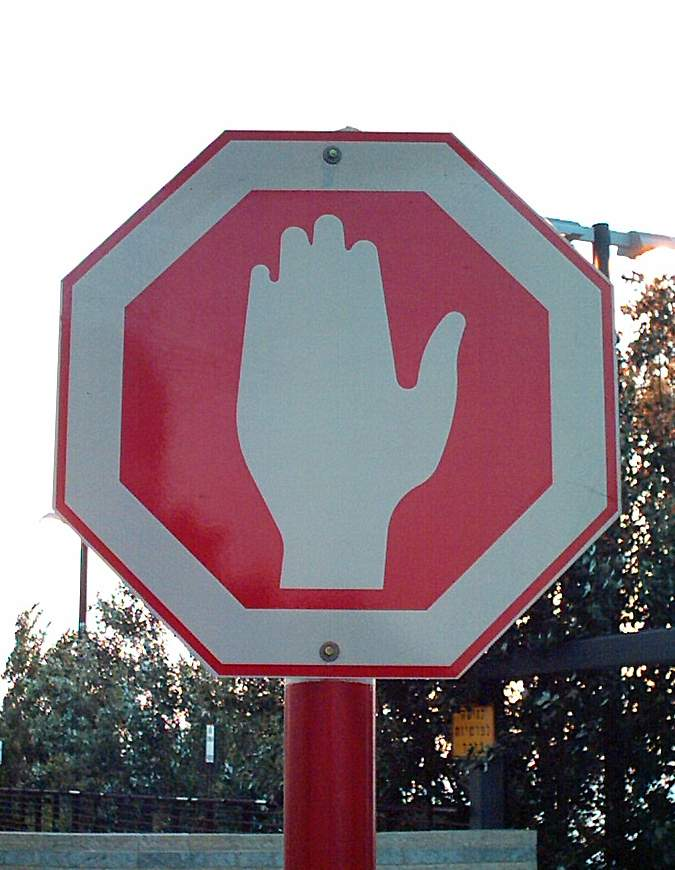
\includegraphics[width=\linewidth,height=0.18\textheight,keepaspectratio]{figures/textvqa_sample_stop_sign.jpg}
        \caption{TextVQA}
    \end{subfigure}
    \hfill
    \begin{subfigure}{0.31\linewidth}
        \centering
        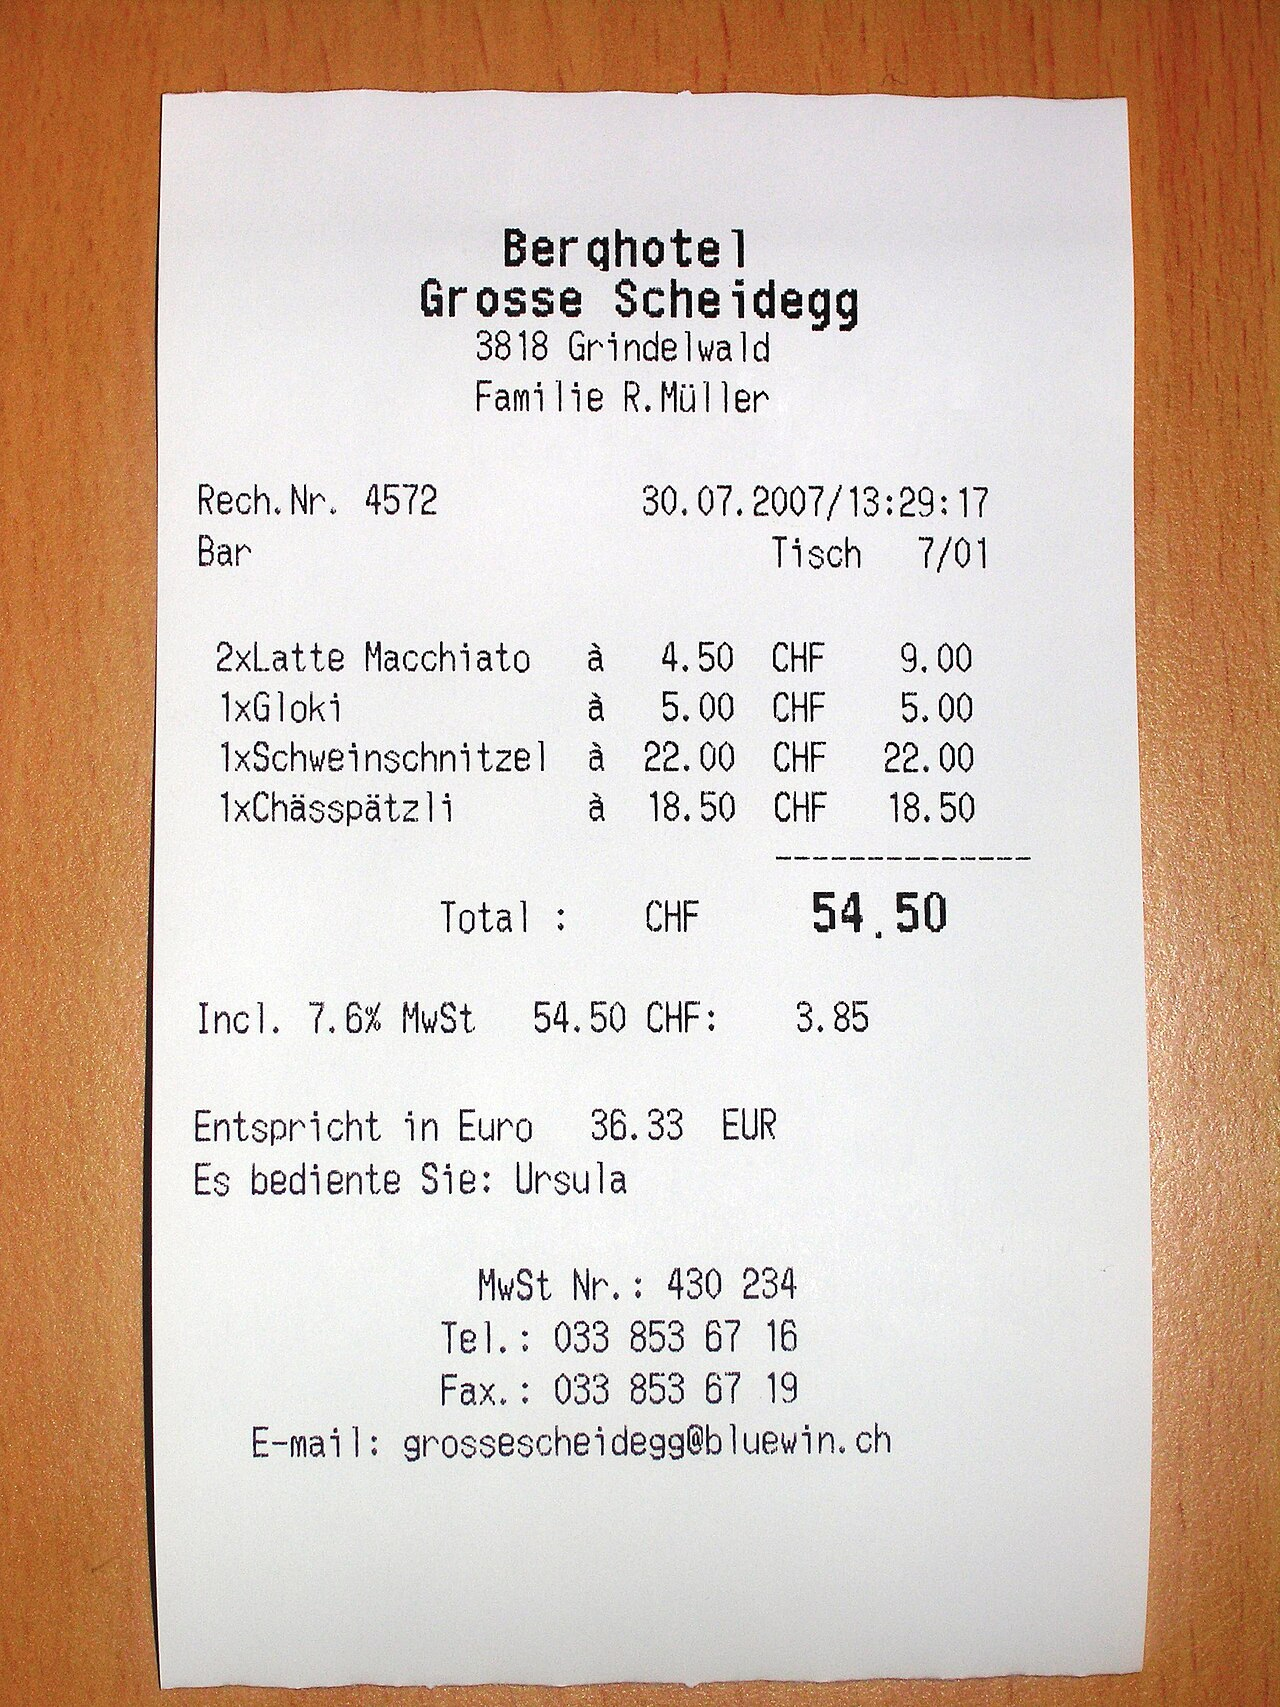
\includegraphics[width=\linewidth,height=0.18\textheight,keepaspectratio]{figures/docvqa_sample_receipt.jpg}
        \caption{DocVQA}
    \end{subfigure}
    \hfill
    \begin{subfigure}{0.31\linewidth}
        \centering
        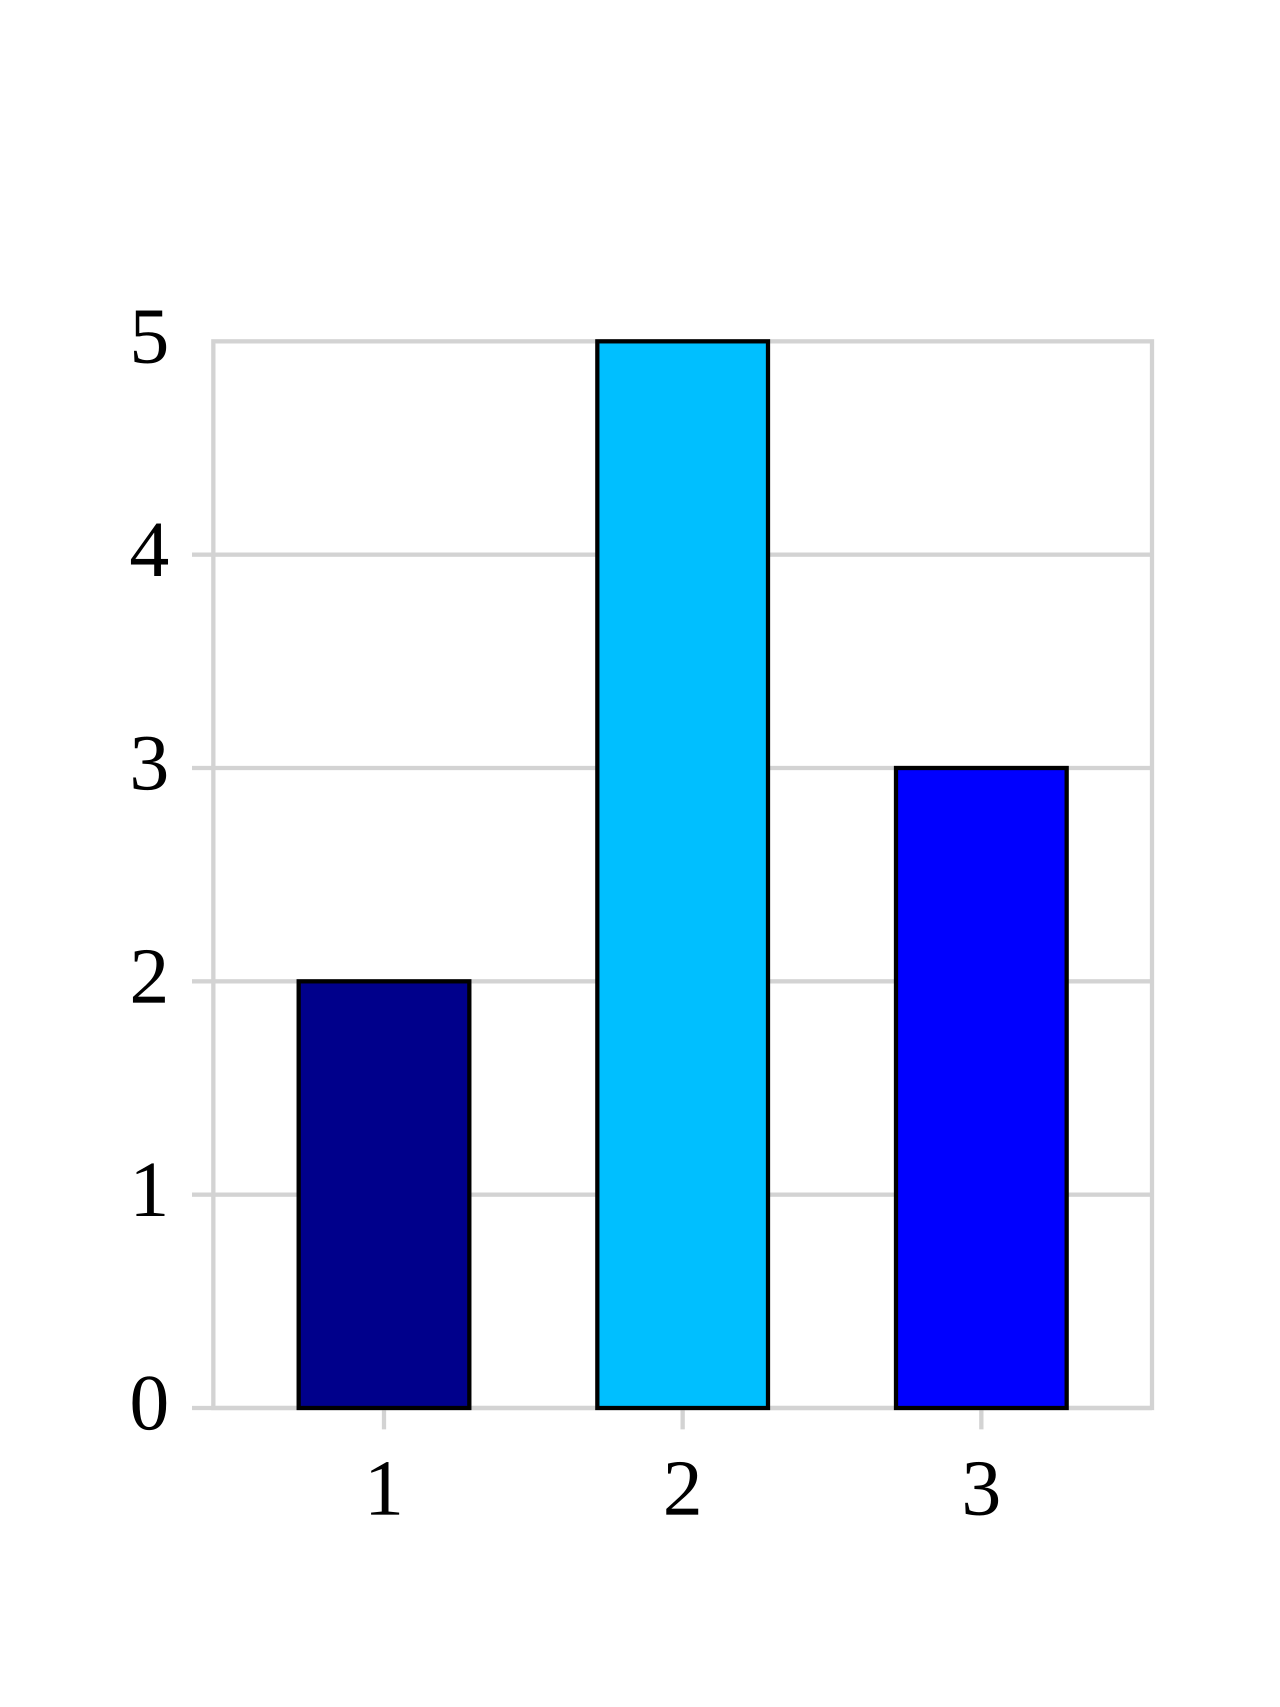
\includegraphics[width=\linewidth,height=0.18\textheight,keepaspectratio]{figures/chartqa_sample_bar_chart.png}
        \caption{ChartQA}
    \end{subfigure}
    \caption[Representative dataset examples.]{Representative dataset examples.\textsuperscript{\thefootnote}}
    \label{fig:dataset-samples}
\end{figure}
\footnotetext[\value{footnote}]{Images adapted from Wikimedia Commons sources~\cite{wikimedia_stop_sign_image,wikimedia_receipt_swiss_image,wikimedia_bar_chart_image}.}

Figure~\ref{fig:dataset-samples} shows the visual differences behind this
benchmark choice. The TextVQA panel represents natural-image reading, where the
relevant cue is embedded in an object in the scene. The DocVQA panel is a
receipt with fields, item rows and totals arranged by document layout. The
ChartQA panel is a bar chart, where answering requires comparing bar heights
and reading values from the plot structure. The evaluation therefore covers
natural scene text, document layouts and chart reasoning. The split sizes used
throughout the evaluation chapter are listed in Table~\ref{tab:dataset-sizes}.
\begin{table}[H]
\centering
\caption[Dataset split sizes.]{Dataset split sizes.}
\label{tab:dataset-sizes}
\scalebox{0.96}{
\begin{tabular}{lrrrr}
\toprule
\textbf{Dataset} & \textbf{Train} & \textbf{Val} & \textbf{Test} & \textbf{Total} \\
\midrule
TextVQA & 34,602 & 5,000 & 5,734 & 45,336 \\
DocVQA & 39,463 & 5,349 & 5,188 & 50,000 \\
ChartQA-H (human) & 7,398 & 960 & 1,250 & 9,608 \\
ChartQA-M (machine) & 20,901 & 960 & 1,250 & 23,111 \\
ChartQA (H+M, combined) & 28,299 & 1,920 & 2,500 & 32,719 \\
\bottomrule
\end{tabular}
}
\end{table}

\section{Training Configuration}

Before training, all benchmark samples are converted into a unified
\textbf{LLaVA-style multimodal instruction format}
\cite{liu2023visualinstructiontuning}. Each example is stored as an image plus
a short user-assistant dialogue, as shown in Listing~\ref{lst:llava-format},
so TextVQA, DocVQA and ChartQA can share the same data loader, prompt template
and answer supervision interface. This format is useful because the model sees
every task as the same conditional generation problem: given an image and a
natural-language user query, generate the assistant answer. It also separates
the visual input path from the textual instruction path while keeping the
answer span explicit, which makes it easier to mask prompt tokens, compute
supervised loss only on assistant tokens and align teacher logits with the same
answer positions during distillation.

\begin{lstlisting}[basicstyle=\ttfamily\footnotesize,breaklines=true,frame=single,caption={Representative LLaVA-style sample used after dataset conversion.},label={lst:llava-format}]
{
  "image": "sample_000123.jpg",
  "conversations": [
    {"from": "human", "value": "<image>\nWhat is the invoice number?"},
    {"from": "gpt", "value": "4572"}
  ]
}
\end{lstlisting}

We run all training jobs on a single high-memory \textbf{NVIDIA H200}
graphics processing unit (GPU) or on comparable single-GPU \textbf{Vast.ai}
instances, depending on availability.
Distillation training uses \textbf{DeepSpeed ZeRO Stage 2}, \textbf{Brain
Floating Point 16 (bf16)} mixed precision, \textbf{TensorFloat-32 (TF32)}
matrix multiplication and gradient checkpointing to control memory use while
keeping the student fully trainable and all teachers frozen
\cite{rajbhandari2020zero,chen2016sublinear}. Full optimization and routing
parameter values are reported in Appendix~\ref{app:experiment-parameters},
Table~\ref{tab:experiment-parameters}. Teacher-logit storage and remote caching
are documented in Appendix~\ref{app:offline-teacher-logit-preparation} and
Appendix~\ref{app:remote-logit-streaming} for reproducibility purposes.

\section{Evaluation Metrics}
We report benchmark-specific official metrics for each dataset.

\textbf{TextVQA.}
For TextVQA, we report the official VQA Accuracy metric. For a predicted
answer \(\hat{a}\), the per-question score is
\[
s_{\text{VQA}}=\min\left(\frac{\#\text{annotators that provided } \hat{a}}{3},\,1\right),
\]
and the final score is the mean over all questions \cite{singh2019vqamodelsread}.

\textbf{DocVQA.}
We report ANLS, the Average Normalized Levenshtein Similarity. The final ANLS
is the average score over all samples
\cite{mathew2021docvqadatasetvqadocument}:
\[
\mathrm{NLS}(a,\hat{a})=1-\frac{d_{\text{Lev}}(a,\hat{a})}{\max(|a|,|\hat{a}|)}, \quad
s_{\text{ANLS}}=
\begin{cases}
\mathrm{NLS}(a,\hat{a}), & \mathrm{NLS}\ge 0.5,\\
0, & \text{otherwise}.
\end{cases}
\]

\textbf{ChartQA.}
For ChartQA, we report Relaxed Accuracy \cite{masry2022chartqabenchmarkquestionanswering}.
A prediction is correct if it matches exactly for text answers. For numeric
answers, the score handles the zero-target case explicitly:
\[
s_{\mathrm{ChartQA}}=
\begin{cases}
\mathbf{1}[\hat{y}=y], & y=0,\\
\mathbf{1}\!\left[\frac{|\hat{y}-y|}{|y|}\le 0.05\right], & y\ne0.
\end{cases}
\]

\section{Baselines and Compared Methods}

For consistency with Chapter~\ref{chap:experiment-results}, we organize the
compared methods into four groups: non-distillation references, same-family
distillation baselines, different-family single-teacher baselines and
heterogeneous teacher baselines. Before introducing the method-specific baselines, the role of each baseline
family is grouped in Table~\ref{tab:baseline-groups}. The grouping separates
student-only references, same-family KD, tokenizer-mismatched single-teacher
transfer and heterogeneous teacher methods.

\begin{table}[tp]
\centering
\caption[Baseline groups.]{Baseline groups.}
\label{tab:baseline-groups}
\small
\setlength{\tabcolsep}{5pt}
\renewcommand{\arraystretch}{1.08}
\begin{tabular}{@{}
  >{\raggedright\arraybackslash}p{0.18\linewidth}
  >{\raggedright\arraybackslash}p{0.24\linewidth}
  >{\raggedright\arraybackslash}p{0.24\linewidth}
  >{\raggedright\arraybackslash}p{0.26\linewidth}@{}}
\toprule
\textbf{Group} & \textbf{Methods} & \textbf{Teacher setup} & \textbf{Purpose} \\
\midrule
Non-distillation references & Original, full finetuning & No teacher & Student-only reference points \\
\midrule
Same-family baselines & Forward KL, Reverse KL, Jensen-Shannon & SmolVLM2-2.2B-Instruct & Standard single-teacher objectives within the SmolVLM family \\
\midrule
Cross-family single-teacher & ULD & Qwen2-VL-2B-Instruct & Cross-family transfer without routed teacher selection \\
\midrule
Heterogeneous teacher baselines & Uniform averaging, SHM-CKA, REINFORCE, \textbf{\methodname{} (Ours)} & Mixed teacher set from multiple VLM families & Static averaging vs. hidden-state matching vs. adaptive teacher assignment \\
\bottomrule
\end{tabular}
\end{table}

The non-distillation references consist of the original student and the
full-finetuning baseline, which provide student-only reference points. The
same-family baselines use \textbf{SmolVLM2-2.2B-Instruct} as teacher for
forward KL, reverse KL and Jensen-Shannon distillation, isolating standard
teacher-student transfer when the tokenizer and output space are matched
\cite{smolvlm2_modelcard,marafioti2025smolvlm,hinton2015distillingknowledgeneuralnetwork,lin1991jensen,cui2024sinkhorn}.
The different-family single-teacher setting uses ULD with a teacher outside
the SmolVLM family, testing tokenizer-mismatched transfer without teacher routing
\cite{boizard2024towardscrosstokenizerdistillation}. The heterogeneous
teacher setting compares uniform averaging, SHM-CKA, REINFORCE and
\methodname{} over a mixed teacher pool, separating static averaging,
hidden-state matching and adaptive teacher assignment
\cite{takezawa2021supervisedtreewasserstein,zhang2023adaptivemultiteachermetalearning,yu2024selectdistill,dasgupta2025improving}.

For the trainable competitor methods, we keep the supervised term
\(\mathcal{L}_{CE}\). The logits-only baselines differ only in the KD signal,
but SHM-CKA also adds a hidden-state alignment term and REINFORCE
also adds a REINFORCE-style policy term
\cite{kornblith2019similarityrepresentations,williams1992simple,yuan2020reinforcedmultiteacherselection}.
In the descriptions below, \(\gamma\) denotes a generic KD mixing coefficient.
\(\alpha_{\mathrm{KD}}\) is reserved for the \methodname{} training objective
as defined in Equation~\ref{eq:final-objective}.

\textbf{Original.} Directly evaluates the released student without
additional optimization, thereby measuring the native capability of the student
model before task adaptation or any teacher-guided distillation signal.

\textbf{Full finetuning.} Optimizes only \(\mathcal{L}_{CE}\) and uses no teacher, which
isolates the effect of supervised task adaptation from any teacher-guided
distillation signal.

\textbf{Forward KL.} Uses
\(\mathcal{L}_{KD}=\mathrm{KL}(p_t\|p_s)\) for same-family soft-target
distillation when teacher and student vocabularies are aligned
\cite{hinton2015distillingknowledgeneuralnetwork}.

\textbf{Reverse KL.} Uses \(\mathcal{L}_{KD}=\mathrm{KL}(p_s\|p_t)\)
\cite{cui2024sinkhorn,wen2023fdistill} as a student-centered divergence
baseline, which tests whether matching the teacher from the student's current
distribution is suitable for VLM distillation. Because the reverse-KL gradient
is weighted by \(p_s\), this objective tends to emphasize regions where the
student already assigns probability.

\textbf{Jensen-Shannon.} Uses the symmetric divergence
\[
\frac{1}{2}\mathrm{KL}(p_s\|m)+\frac{1}{2}\mathrm{KL}(p_t\|m),
\qquad
m=\frac{1}{2}(p_s+p_t).
\]
It tests whether a bounded symmetric objective is more stable than KL
\cite{lin1991jensen,cui2024sinkhorn}.

\textbf{ULD.} Uses \(\mathcal{L}_{KD}=\|\pi(p_s)-\pi(p_t)\|_1\)
\cite{boizard2024towardscrosstokenizerdistillation}. This is the main
tokenizer-mismatched logits baseline because it compares ranked probability mass,
not token IDs.

\textbf{SHM-CKA.} Extends ULD with a hidden-state CKA penalty
\cite{boizard2024towardscrosstokenizerdistillation,dasgupta2025improving,kornblith2019similarityrepresentations}.
For the heterogeneous setting, both the ULD and layer-matching terms are
averaged uniformly across teachers before combining with \(\mathcal{L}_{CE}\).
Full implementation details are given in
Appendix~\ref{app:baseline-implementation-details}.

\textbf{Uniform multi-teacher.} Assigns fixed equal weights to all teachers
in the heterogeneous pool,
\(\mathcal{L}_{KD}=\frac{1}{M}\sum_{i=1}^{M}\mathcal{L}_{KD}^{(i)}\)
\cite{yuan2020reinforcedmultiteacherselection,zhang2023adaptivemultiteachermetalearning},
thereby testing whether teacher diversity alone is sufficient without adaptive
routing or gradient-aware weighting.

\textbf{REINFORCE.} Replaces deterministic routing with a stochastic policy
that samples teachers and updates the selector with REINFORCE
\cite{williams1992simple,yuan2020reinforcedmultiteacherselection}, providing
an adaptive routing baseline that does not use the gradient-agreement
refinement introduced by \methodname{}.
The selector is trained with the policy-gradient term
\begin{equation}
\mathcal{L}_{\mathrm{pol}}
=
-(r-b)\log p(\mathbf{m}\mid\boldsymbol{\pi}),
\end{equation}
where \(r\) is the reward, \(b\) is an EMA reward baseline and
\(\mathbf{m}\) is the sampled teacher mask. Its final training objective is
\begin{equation}
\mathcal{L}_{\mathrm{RS}}
=
\mathcal{L}_{CE}
+ \gamma \mathcal{L}_{KD}
+ \lambda_{\pi}\mathcal{L}_{\mathrm{pol}}.
\end{equation}
Additional baseline implementation details are reported in
Appendix~\ref{app:baseline-implementation-details}.


\section{Ablation Settings}
\label{sec:ablation-settings}

The ablation study in Section~\ref{sec:ablation} isolates the main components
of \methodname{} on DocVQA while keeping the teacher set and training protocol
close to the final method. The variants change one mechanism at a time so that
the result table can separate teacher diversity, sparse routing,
gradient-agreement weighting and EMA score smoothing.
The effect of EMA smoothing is isolated in the \(\beta_{\mathrm{EMA}}=0\)
ablation in Section~\ref{sec:ablation}.

\textbf{Cross-family ULD.} The single-teacher cross-family baseline uses one teacher outside the SmolVLM
family and optimizes
\[
\mathcal{L}
=
\mathcal{L}_{CE}
+
\alpha_{\mathrm{KD}}\mathcal{L}_{ULD},
\qquad
\mathcal{L}_{ULD}
=
\|\pi(p_s)-\pi(p_t)\|_1 .
\]

\textbf{Uniform averaging.} The uniform variant adds the full heterogeneous teacher pool but assigns fixed
equal weights:
\[
\mathcal{L}
=
\mathcal{L}_{CE}
+
\alpha_{\mathrm{KD}}\frac{1}{M}\sum_{i=1}^{M}\mathcal{L}_{TW}^{(i)}.
\]
This setting tests whether teacher diversity alone is enough without adaptive
selection.

\textbf{Routing only.} The routing-only variant keeps sparse teacher selection but replaces
post-routing weights with uniform weights within the routed set:
\[
w_i^{(b)}
=
u_i^{(b)}
=
\frac{\mathbf{1}[i\in\mathcal{R}_b]}{|\mathcal{R}_b|}.
\]
This setting tests whether top-\(k\) routing is useful without
gradient-agreement refinement.

\textbf{Full GRACE.} The full method combines trie-Wasserstein KD, sparse routing and
gradient-agreement weighting:
\[
w_i^{(b)}
\propto
(\hat p_i^{(b)})^{\lambda_{\mathrm{blend}}}
(\omega_i^{(b)})^{1-\lambda_{\mathrm{blend}}}.
\]
Two additional ablation variants isolate the final weighting mechanism,
reported in Table~\ref{tab:docvqa-planned-ablation}. The
\(\lambda_{\mathrm{blend}}=1.0\) variant keeps the active-set threshold and
fallback rules but removes the score-softmax factor from the confident-score
case:
\[
w_i^{(b)}
\propto
\hat{p}_i^{(b)}\mathbf{1}[i\in\mathcal{A}_b].
\]
This row is an active-set-restricted router-weight ablation, not a pure
router-only ablation over all routed teachers. The \(\beta_{\mathrm{EMA}}=0\)
variant removes temporal smoothing by setting \(\hat{s}_i=s_i\) before
score-softmax weighting.

The training runs reported in this thesis rely on an offline teacher-logit
preparation step and a remote logit-streaming infrastructure that are
separate from the fair-comparison protocol described above. Teacher logits are
generated once and stored on Cloudflare R2. During training, they are streamed
lazily through a 100~GB local cache without copying the full logit store locally.
Full engineering
details, including the caching script, path conventions, streaming loader and
the logit-streaming settings table, are given in
Appendix~\ref{app:offline-teacher-logit-preparation} and
Appendix~\ref{app:remote-logit-streaming}.
\newpage\cleardoublepage
\chapter{Experiment Results}
\label{chap:experiment-results}

\section{Main Comparison Results}
This section compares the proposed method with the baselines on TextVQA, DocVQA and ChartQA.

\subsection{Baseline Results}
Before applying any adaptation or distillation, we report the original performance of the two base student models, \textbf{SmolVLM-500M} and \textbf{SmolVLM-256M}. These baseline results establish the starting point for later comparison. All results are obtained using \textbf{VLM-Eval-Kit} under the same evaluation pipeline described in Chapter~\ref{chap:evaluation-methodology}.

\begin{table}[htbp]
\centering
\begin{tabular}{lccc}
\toprule
\textbf{Model} & \textbf{TextVQA} & \textbf{DocVQA} & \textbf{ChartQA} \\
\midrule
SmolVLM-500M & 56.75 & 59.5247 & 62.8 \\
SmolVLM-256M & 47.17 & 48.6411 & 45.04 \\
\bottomrule
\end{tabular}
\caption{Original benchmark results of the two SmolVLM models evaluated with VLM-Eval-Kit.}
\label{tab:smolvlm-original-results}
\end{table}

\section{Ablation Study}
This section analyzes the effect of teacher-set selection, weighting strategy and student model size on final performance.

\section{Qualitative Analysis}
This section presents representative examples to inspect how distillation affects text reading and basic reasoning behavior.

\section{Discussion}
This section discusses the trade-off between model size, teacher supervision and transfer performance across the evaluated benchmarks.
\newpage\cleardoublepage
\chapter*{Conclusion and Future Work}
\phantomsection
\addcontentsline{toc}{chapter}{Conclusion and Future Work}

\section*{Summary}
\phantomsection
\addcontentsline{toc}{section}{Summary}
This thesis studied knowledge distillation for heterogeneous vision-language
models where teachers vary in usefulness across samples and differ from the
student in tokenizer. Building on cross-tokenizer distillation, optimal transport and
sparse routing
\cite{boizard2024towardscrosstokenizerdistillation,peyre2019computationaloptimaltransport,fedus2022switchtransformersscalingtrillion},
the work introduced \gracefull{} (\gracename{}), a routed multi-teacher
framework that combines three main contributions: Byte-Trie Wasserstein
tokenizer-agnostic distillation, sparse top-\(k\) teacher routing and gradient-agreement
refinement.

Byte-Trie Wasserstein distillation maps decoded teacher and student tokens
into a shared byte-trie structure and compares subtree probability masses
across tokenizer vocabularies. The objective-aware refinement combines sparse
routing, which selects teachers relevant to each sample, with gradient-agreement
reweighting by the cosine alignment between each teacher's KD gradient and the
supervised answer gradient. The empirical evaluation on TextVQA, DocVQA and
ChartQA shows that this combination outperforms same-family, single-teacher
and heterogeneous multi-teacher baselines.

Across TextVQA, DocVQA and ChartQA, \methodname{} scores highest among the
compared methods in Chapter~\ref{chap:experiment-results}. For
SmolVLM-500M, it reaches 69.38 on TextVQA, 73.11 on DocVQA and 80.20 on
ChartQA. For SmolVLM-256M, it reaches 60.73, 60.48 and 72.32 on the same three
benchmarks. On SmolVLM-500M, \methodname{} closes about 55\% of the original
teacher-student gap on TextVQA and ChartQA and about 40\% on DocVQA.
Closing more than half the gap to teachers six times larger suggests that
the supervision design, rather than model capacity, is the primary bottleneck
for compact VLMs on these benchmarks.

\section*{Limitations}
\phantomsection
\addcontentsline{toc}{section}{Limitations}
Three limitations qualify the current results. \textbf{Cost-limited evaluation.} The reported
single-run design limits uncertainty analysis for small gaps between
high-scoring baselines because confidence intervals and estimates from repeated runs are unavailable. As reported in
Section~\ref{sec:efficiency-analysis}, an average run costs approximately
14.41 USD before offline cache generation and storage cost. Although the main
tables use a shared four-teacher pool and consistent hyperparameters, no uncertainty estimates are available for closely matched methods. Small score differences between high-scoring baselines should be treated with caution until repeated-run estimates are available.

\textbf{Scope of validation.} The empirical study focuses on
VQA benchmarks and SmolVLM-family students. The results support VQA
distillation with compact projector-based students, while broader multimodal
task families, other student architectures and larger teacher pools require
further validation. Tasks with long-form answers, multi-image inputs, video reasoning or
open-ended dialogue require different forms of teacher selection and answer
supervision.

\textbf{Reasoning-oriented model support remains outside the current scope.}
GRACE currently distills teacher supervision through output distributions at answer tokens
and gradient agreement with the supervised answer loss. This design fits the evaluated VQA setting, where the target is a short final
answer. It focuses on supervision of final answers and
leaves intermediate deliberation traces, hidden reasoning tokens and extended
test-time reasoning for future work. If a teacher produces only a final answer
distribution, GRACE can still use that distribution as a teacher signal. Future
extensions should separate tokens in the reasoning phase from those in the
answer phase, route teachers by the quality of intermediate reasoning, and
define distillation objectives for multi-step reasoning traces.

\section*{Future Work}
\phantomsection
\addcontentsline{toc}{section}{Future Work}
Four directions remain. The most immediate gap is statistical: repeated runs
with multiple random seeds would clarify which score differences between close
multi-teacher baselines are reliable. On the systems side, more compact logit
storage, adaptive cache loading and lower-cost agreement scoring would reduce
the cost of scaling the method to larger datasets and teacher pools. Beyond
output-level supervision, visual token alignment, cross-attention transfer and
region-level matching could complement the current KD signal for tasks where
the student must localize evidence before answering. Reasoning-oriented models
raise a harder problem: distinguishing reasoning-phase tokens from
final-answer tokens and specifying how teachers are selected when intermediate
traces are available. Router input features, principled conflict resolution and
teacher pools that combine specialized document, chart, general VLM and
reasoning-oriented models are additional open questions
\cite{yuan2020reinforcedmultiteacherselection,zhang2023adaptivemultiteachermetalearning,yu2024selectdistill}.
\newpage\cleardoublepage

%\nocite{*}
\phantomsection
\addcontentsline{toc}{chapter}{References}
\bibliography{references}\newpage\cleardoublepage

\appendix
\renewcommand{\appendixname}{Appendix}
\addtocontents{toc}{\protect\renewcommand{\protect\cftchappresnum}{Appendix }}
\addtocontents{toc}{\protect\setlength{\protect\cftchapnumwidth}{6.5em}}
\titleformat{\chapter}[display]
{\normalfont\huge\bfseries}{Appendix \thechapter}{0pt}{\LARGE}
\input{chapters/appendix_tree_wasserstein}\newpage\cleardoublepage
\input{chapters/appendix_experiment_parameters}\newpage\cleardoublepage
\addtocontents{toc}{\protect\renewcommand{\protect\cftchappresnum}{Chapter }}

\end{document}
